\documentclass[journal]{IEEEtran}
\usepackage{graphicx}
\graphicspath{{figures/}}
\usepackage{amsmath, amssymb}
\usepackage{booktabs}
\usepackage{multirow}
\usepackage{makecell}
\usepackage{array}
\usepackage[colorlinks=false,hidelinks]{hyperref}

\begin{document}

\title{MARS: A Reconfigurable Accelerator Architecture with Runtime Task Switching for Ultra-Low-Bit Streaming Inference}

\author{Po-Chun~Huang, Pao-Ann~Hsiung, and~Chun-Hsien~Huang%
\thanks{Po-Chun Huang and Pao-Ann Hsiung are with the Department of Computer Science and Information Engineering, National Chung Cheng University, Chiayi, Taiwan. Chun-Hsien Huang is with the Department of Electrical Engineering, National Chung Cheng University, Chiayi, Taiwan.}}

\maketitle

\begin{abstract}
Edge FPGA platforms must serve multiple AI tasks under tight resource budgets. The surveyed PR-based CNN methods require a reconfiguration controller and per-task partial bitstreams with millisecond-scale switch latencies, while fixed-feature-extractor designs cannot adapt the feature extractor at runtime. Combining ultra-low-bit quantisation with parameter-efficient transfer learning (PEFT) on a streaming dataflow accelerator could resolve this, but we observe a pronounced degradation of single-branch adapter effectiveness specifically at 1 bit. This paper presents MARS (Multi-Branch Adapter Reconfigurable Streaming-accelerator), an ultra-low-bit FPGA accelerator that integrates a custom Adapter IP into a streaming-dataflow backbone. MARS uses multi-branch adapter scaling to recover part of the transfer accuracy lost under binarisation, a Residual Correction (RC) term---the adapter's pre-existing down-projection bias, realised at zero additional arithmetic or datapath cost, with its storage counted in the adapter budget---to mitigate the pronounced 1-bit-specific degradation, and a runtime configuration interface that reprograms all task-dependent parameters over a single bitstream without any fabric reconfiguration. On a frozen 1-bit VGG-like backbone, multi-branch scaling raises transfer accuracy by $+3.4$ percentage points on average (up to $+11.3$) across twenty backbone--target pairs in the deployed-geometry sweep, and RC contributes up to $+23.0$~pp. On a PYNQ-Z2, the compactness build switches at runtime among five task-specific models with on-board accuracy within $0.69$~pp of software and a $1.86$~ms per-task configuration rewrite ($\approx$25~KB) with verified post-switch correctness; a throughput-oriented build sustains 1{,}866~img/s at 2.214~W (842.7~img/s/W) on a protocol-matched 1W1A workload with deployment-representative, different adapter geometries (Vivado-estimated FPGA power vs.\ measured GPU power).
\end{abstract}

\begin{IEEEkeywords}
Parameter-efficient transfer learning, ultra-low-bit quantisation, FPGA accelerator, streaming dataflow, runtime task switching, residual correction.
\end{IEEEkeywords}

\section{Introduction}
\IEEEPARstart{E}{dge} FPGA accelerators are increasingly asked to serve several AI tasks from one device: a drone alternates between navigation and object recognition; a smart camera switches between day-time and infra-red models. On FPGAs, the prevailing answer is partial reconfiguration (PR): each task is compiled into a partial bitstream, and a fabric-reconfiguration controller swaps hardware regions at run time~\cite{Huang2024ACNNE,Rangsikunpum2024CoarseToFine}. PR works, but it carries a fixed tax---a reconfiguration controller, a per-task bitstream repository that grows linearly with the task count, and measured switch latencies from $5.2$~ms (ZyCAP) up to $97$--$114$~ms (PCAP) on PYNQ-class devices. The alternative family fixes a feature extractor in the fabric and swaps only back-end logic~\cite{Whatmough2019FixyNN} or selects among variants resident on chip~\cite{ElBouazzaoui2025NeuroAdaptive}; these avoid fabric rewrites but freeze the reachable task set at synthesis time.

A third path is suggested by parameter-efficient transfer learning (PEFT)~\cite{Houlsby2019Adapters,Hu2022LoRA,Yu2024VisualTuning}: keep one shared backbone frozen and adapt tasks through small inserted modules such as Conv-Adapter~\cite{Chen2024ConvAdapter}. If the backbone is also quantised to the 1-bit weight, 1-bit activation (1W1A) regime~\cite{Rastegari2016XNOR,Hubara2016BinarizedNN,Qin2020BNNSurvey} and mapped to a streaming dataflow architecture~\cite{Umuroglu2017FINN,Blott2018FINNR}, then a task switch reduces to rewriting a small set of parameters---no fabric reconfiguration at all. However, in the evaluated VGG-like configurations, a single binary adapter branch exhibits a substantially larger transfer-accuracy degradation at 1W1A than at 2--8 bits, echoing the precision-redundancy perspective of~\cite{Jie2023PrecisionRedundancy}.

This paper presents \textbf{MARS} (Multi-Branch Adapter Reconfigurable Streaming-accelerator), which makes the ultra-low-bit adapter path practical and carries it through to an on-board-verified system. Our contributions are:
\begin{enumerate}
\item \textbf{A 1-bit-specific empirical finding and its hardware-efficient mitigation.} The down-convolution bias of Conv-Adapter, isolated here as a Residual Correction (RC) term, has a substantially larger measured effect at 1W1A: it contributes up to $+23.0$~pp on CIFAR-10$\to$SVHN in the deployed geometry, whereas its effect at 2--8 bits is typically within $\pm 0.3$~pp (at most $1.4$~pp). RC is realised at zero additional arithmetic or datapath cost by folding it into the accumulator initial value, with its storage and configuration bytes counted in the adapter budget.
\item \textbf{Multi-branch adapter scaling.} Summing $M$ independently-parameterised binary branches increases the effective capacity of the binary adapter path, raising 1-bit transfer accuracy by $+3.36$~pp on average (up to $+11.33$~pp) across twenty backbone--target pairs in the single-seed deployed-geometry sweep.
\item \textbf{Single-bitstream runtime task switching.} A 19-LUT AXI-Lite Function Switch Controller reprograms all task-dependent parameters ($\approx$25~KB per task) at run time; on-chip cost is $O(1)$ in the number of same-backbone, same-input-size, same-output-head classification tasks.
\item \textbf{On-board verification with explicit evidence boundaries.} A compactness build switches at runtime among five task-specific models on one PYNQ-Z2 bitstream, each within $0.69$~pp of its software reference, with a $1.86\pm0.04$~ms configuration rewrite (post-switch correctness verified); a throughput build sustains 1{,}866~img/s at 2.214~W on a matched 1W1A workload. Multi-branch configurations beyond $M{=}1$ exceed the XC7Z020 and are verified at the RTL-simulation and post-synthesis levels only.
\end{enumerate}

The remainder of this paper is organised as follows. Section~II reviews the three research threads MARS builds on. Section~III presents the method: the binary adapter, RC, multi-branch scaling, and training. Section~IV details the hardware architecture and the switching mechanism. Section~V reports software, resource, on-board, and cross-platform results with explicit evidence levels, Section~VI states the limitations, and Section~VII concludes.

\section{Related Work}
\subsection{Ultra-Low-Bit FPGA Dataflow Accelerators}
Binarised neural networks replace multiply--accumulate with XNOR--popcount~\cite{Rastegari2016XNOR,Hubara2016BinarizedNN}, and streaming-dataflow compilers such as FINN~\cite{Umuroglu2017FINN,Blott2018FINNR} map every layer to a dedicated matrix--vector--activation unit (MVAU) with on-chip weights, yielding high throughput per watt on small FPGAs~\cite{Gao2025CNNFPGA,Nechi2023FPGADLSurvey}.  Beyond FINN, RTL-level MVAU implementations~\cite{Alam2023RTLMVU}, HPC-oriented extensions~\cite{Jungemann2025FINNHPC}, hls4ml~\cite{Schulte2025hls4ml}, ONNX-to-hardware flows~\cite{Manca2024ONNXtoHW}, and all-on-chip stream accelerators~\cite{Kang2023AoCStream,Zhao2024HighThroughput} broaden the dataflow family, and recent surveys catalogue the design space~\cite{Jiang2025FPGACNNReview,Li2025DataflowTiling,Su2023BNNFPGASurvey,Zhan2023BNNEdge,Antunes2025SpaceSurvey,Liu2024LightweightDLSurvey,Khaki2025OptimizingDL}. On the training side, the line from BinaryConnect~\cite{Courbariaux2016BinaryConnect} through Bi-Real Net and ReActNet~\cite{Liu2018BiReal,Liu2020ReActNet} and FPGA BNN systems such as FP-BNN~\cite{Liang2018FPBNN} improves binary representational capability, while integer-quantisation practice is consolidated in~\cite{Jacob2018Quantization,Nagel2021QuantWhitepaper,Fouda2025QuantCNNHW,Tasci2025FPGAQNN}. These pipelines, however, are compiled for a single task: weights are baked into the bitstream, and serving another task conventionally means another bitstream.

\subsection{PEFT and Adapter Methods}
Adapters~\cite{Houlsby2019Adapters}, LoRA~\cite{Hu2022LoRA}, and their vision descendants~\cite{Yu2024VisualTuning} adapt a frozen backbone with a small number of trained parameters. Conv-Adapter~\cite{Chen2024ConvAdapter} inserts a down-projection/nonlinearity/up-projection bottleneck beside convolutional layers. Edge-oriented PEFT variants for CNNs and IoT devices are emerging~\cite{Ding2024LoRAC,Kwak2025LoRAEdge,Lu2025CacheAdapter}, and benchmarks systematise the method space~\cite{Belanec2025PEFTBench}. Prior PEFT work targets full-precision or moderately quantised models; the 1-bit regime---where the adapter itself must be binary---is largely unexplored, and~\cite{Jie2023PrecisionRedundancy} suggests the precision redundancy available to adapters becomes severely limited at 1 bit.

\subsection{Task Switching on FPGAs}
Published task-switching FPGA inference falls into three families: PR-based systems (ACNNE~\cite{Huang2024ACNNE}, coarse-to-fine PR~\cite{Rangsikunpum2024CoarseToFine}, dynamic PR managers~\cite{Boudjadar2025DynamicFPGA,Kang2025RuntimeRobust}), fixed-feature-extractor designs with per-task back-ends~\cite{Whatmough2019FixyNN}, and on-chip parameter selection among synthesis-time variants~\cite{ElBouazzaoui2025NeuroAdaptive}. To the best of our knowledge among the surveyed FPGA/PEFT accelerator works, no prior system combines an ultra-low-bit shared backbone, feature-extractor-level adapter adaptation, and single-bitstream runtime task switching verified on hardware; MARS fills this gap.

\section{The MARS Method}
\subsection{Background: Streaming 1W1A Pipelines}
In a FINN-style pipeline every layer is a matrix--vector--activation unit: an XNOR array against on-chip 1-bit weights, a popcount, and a thresholding stage that folds BatchNorm and the binary activation into one per-channel integer comparison. Critically, thresholding happens \emph{inside} the MVAU, so the raw partial sum is not normally exposed; any additive per-task correction applied after an MVAU would have to re-quantise an already-binarised signal. This is the architectural obstacle that the Super Wrapper of Section~IV removes, and it is why the adapter must be co-designed with the pipeline rather than appended to it.

\subsection{One-Branch Binary Adapter}
MARS inserts one adapter beside each of the five adapter-hosting convolution layers of a frozen 1W1A VGG-like backbone (the FINN reference CNV network: six convolutional and three fully connected layers, pre-trained on CIFAR-10). For hidden channel $j$ the down-projection accumulates XNOR products of the binary input $x$ with 1-bit weights and adds a per-channel bias:
\begin{equation}
h_j = b_j + \sum_{i=1}^{C_{\text{in}}} \operatorname{XNOR}\bigl(W^{\text{down}}_{j,i}, x_i\bigr), \qquad j = 1, \ldots, C_h,
\label{eq:down}
\end{equation}
where $\operatorname{XNOR}(\cdot,\cdot)$ denotes the bitwise exclusive-NOR and $C_h$ is the bottleneck width. A binary activation $a_j = \mathbb{I}[h_j \ge 0]$ follows, and the up-projection restores the output width:
\begin{equation}
z_o = \sum_{j=1}^{C_h} \operatorname{XNOR}\bigl(W^{\text{up}}_{o,j}, a_j\bigr), \qquad o = 1, \ldots, C_{\text{out}}.
\label{eq:up}
\end{equation}
The deployed geometry uses $1{\times}1$ down-convolutions with $C_h = C_{\text{in}}/4$ and a scalar per-branch scale.

\subsection{Residual Correction (RC)}
The bias term $b_j$ in \eqref{eq:down} is not new---it is the bias Conv-Adapter already has. Our finding is that at 1 bit this term changes character: without it, the binary activation can only cut the popcount distribution at zero, which need not coincide with the decision boundary the task requires; with it, the cut can move toward that boundary---consistent with the ablation, though not itself a verified mechanism. We therefore isolate it as the Residual Correction and keep it explicitly. A small example makes the mechanism concrete. Suppose a hidden channel's popcount over the window ranges over $[0, 64]$ and the task-optimal decision boundary sits at $41$. Without a bias, $\operatorname{sign}(h)$ can only cut at zero of the \emph{centred} accumulation---equivalent to a fixed boundary at $32$---so every sample between $32$ and $41$ lands on the wrong side, and at 1~bit there is no downstream precision to compensate. With RC $=-9$ folded into the accumulation, the cut moves onto the boundary---an illustrative numerical example rather than values extracted from a measured network channel. One plausible explanation for the smaller effect at ${\geq}2$~bits is that additional activation levels preserve magnitude information that downstream layers may exploit; this interpretation is consistent with the ablation but is not directly verified by activation-distribution analysis.

In hardware, RC is folded into the \emph{initial value} of the down-projection accumulator: the accumulator must load an initial value at every output window anyway, so RC replaces the constant zero at zero additional arithmetic, DSP, or pipeline cost; the only real cost is the RC storage and its share of the per-task configuration bytes, which we count in the adapter budget. Fig.~\ref{fig:rc_hw} shows the realisation: \texttt{ram\_rc} drives the initialisation input of the multiplexer in front of the accumulator register, selected by the FSM at every window start, while the remaining cycles follow the accumulate loop---the crossed-out ``+RC'' stage does not exist in the RTL.

\begin{figure}[!t]
\centering
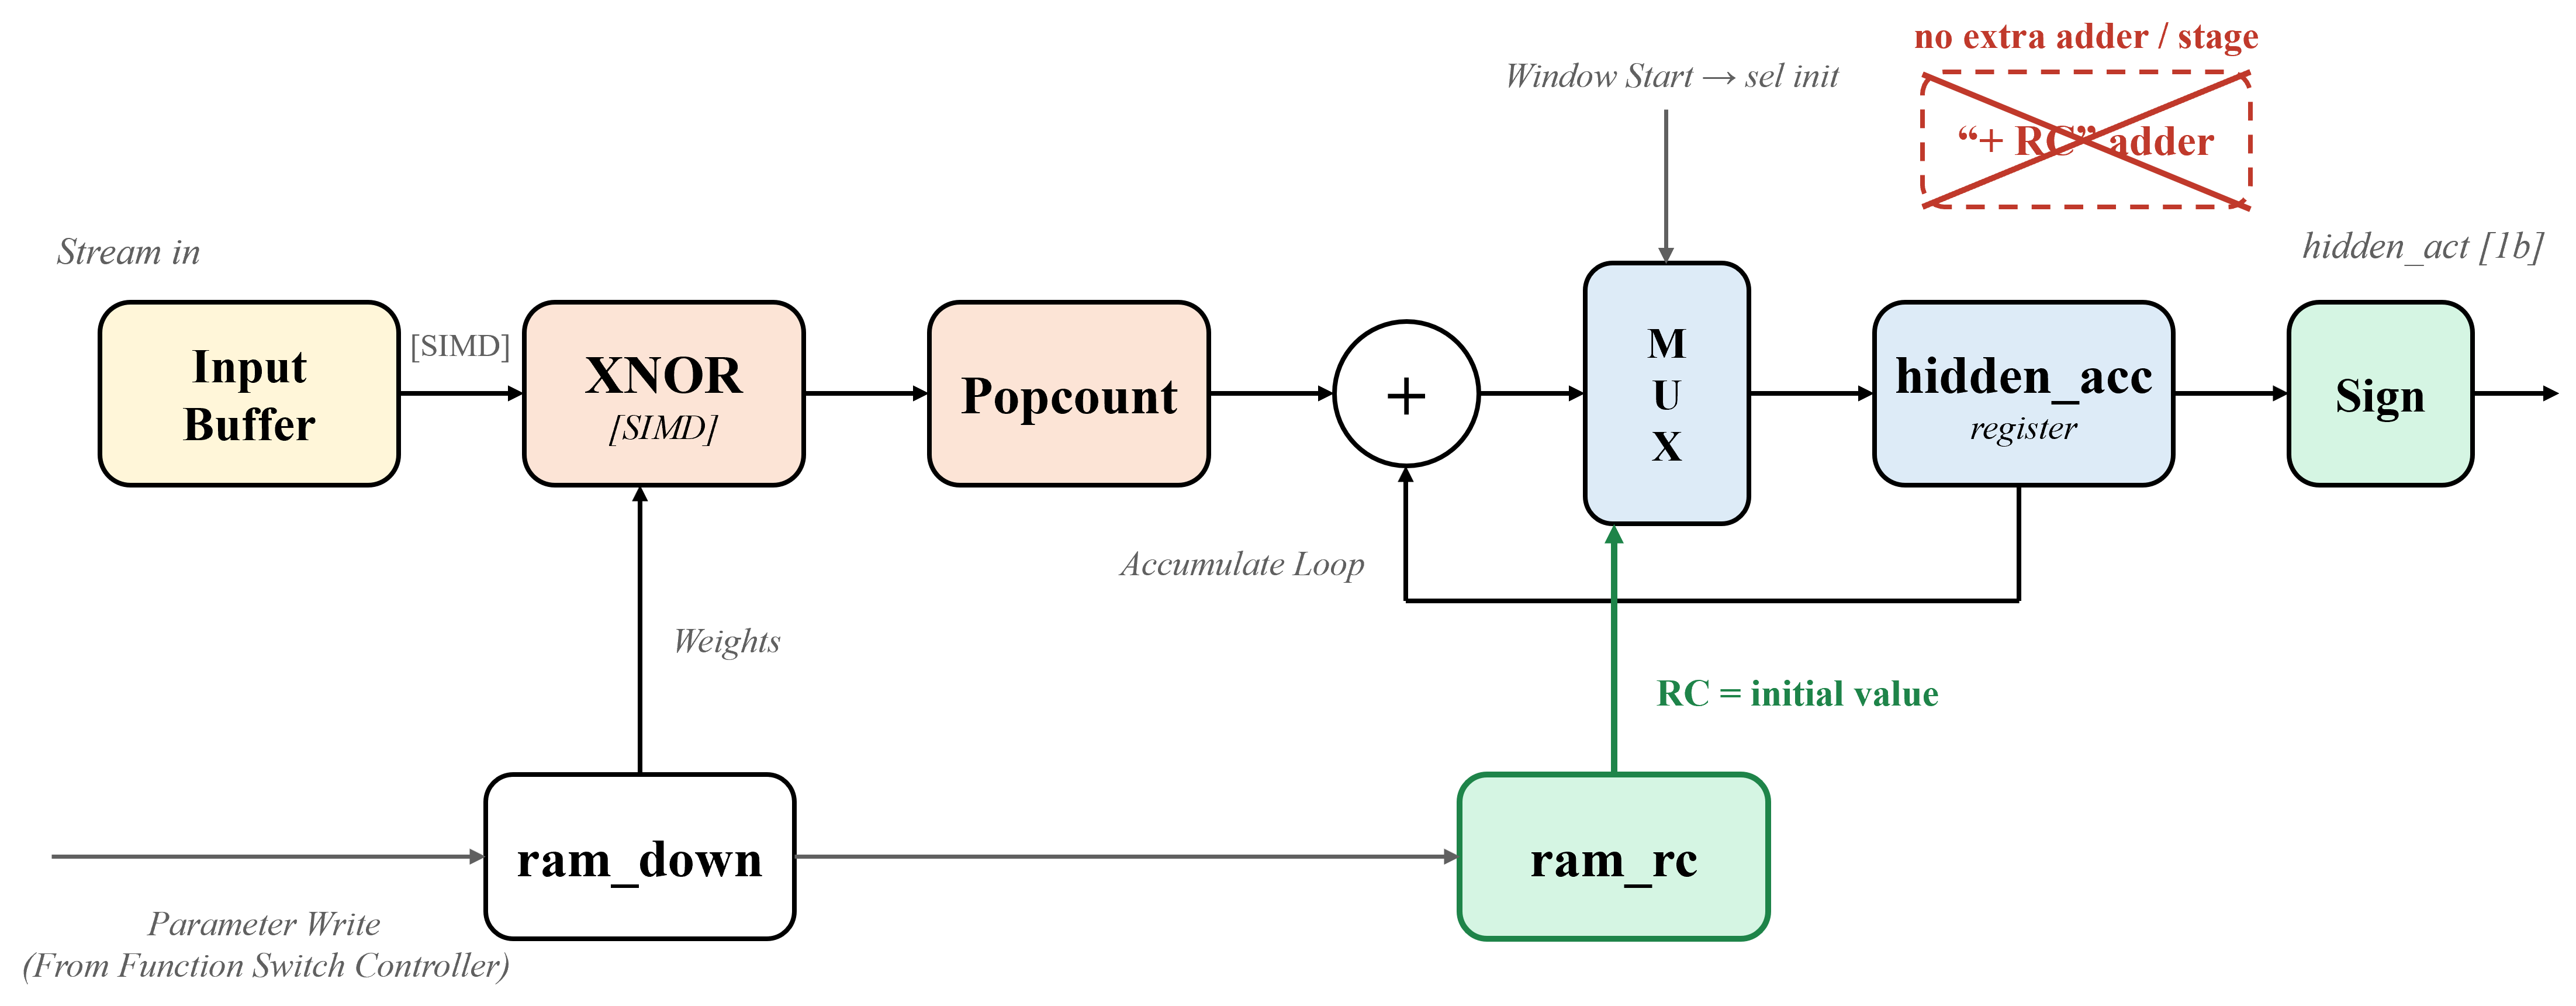
\includegraphics[width=0.92\columnwidth]{rc_in_hardware.png}
\caption{RC in hardware: accumulator initialisation from \texttt{ram\_rc}; no extra adder or pipeline stage.}
\label{fig:rc_hw}
\end{figure}

\subsection{Multi-Branch Adapter}
MARS instantiates $M$ structurally identical branches with independent weights, RC, and scales, and sums them:
\begin{equation}
y_o = \sum_{i=1}^{M} \alpha_i\, z_o^{(i)}, \qquad o = 1, \ldots, C_{\text{out}}.
\label{eq:multibranch}
\end{equation}
Summing independently parameterised branch outputs enriches the set of integer-valued corrections the adapter can express (each branch output is itself a multi-level popcount value, so no fixed output-level count is claimed). The parameter overhead is linear, $\Delta P(M) = M \times 58{,}533$ ($+3.78\%$ of the 1{,}546{,}690-parameter backbone per branch).

\subsection{Wide vs.\ Deployed Geometry}
Two adapter geometries are used deliberately. The \emph{wide} geometry ($3{\times}3$ down-convolution, per-channel $\alpha$, $C_h = C_{\text{out}}/4$) is the software-oriented reference and achieves the highest accuracy on the CIFAR-10 backbone; the \emph{deployed} geometry ($1{\times}1$ down-convolution, scalar $\alpha$, $C_h = C_{\text{in}}/4$) is the configuration carried into the bitstream, chosen because a $1{\times}1$ projection needs no additional line buffering in a streaming pipeline and a scalar $\alpha$ collapses into a single per-layer look-up table. The relative ranking of the two geometries is source-dependent (Section~V), so conclusions involving exact accuracy differences are reported separately for each geometry.

\subsection{Training}
All task-dependent parameters---the $M$ branches and the classifier---are trained jointly, end-to-end, with the backbone frozen. Branch weights are binarised in the forward pass,
\begin{equation}
W^{\text{down},(i)} = \operatorname{sign}\bigl(\widetilde{W}^{\text{down},(i)}\bigr), \quad
W^{\text{up},(i)} = \operatorname{sign}\bigl(\widetilde{W}^{\text{up},(i)}\bigr),
\label{eq:binarise}
\end{equation}
and the backward pass uses the straight-through estimator
\begin{equation}
\frac{\partial \operatorname{sign}(u)}{\partial u} \;\approx\; \mathbf{1}_{|u| \le 1},
\label{eq:ste}
\end{equation}
so ADAM updates the real-valued latent weights and the real-valued RC bias. The per-branch scale $\alpha_i$ multiplies its branch output linearly and receives the exact gradient
\begin{equation}
\frac{\partial L}{\partial \alpha_i} \;=\; \Bigl\langle \frac{\partial L}{\partial y},\; z^{(i)} \Bigr\rangle,
\label{eq:alpha}
\end{equation}
with no estimator involved. Nothing forces the branches apart: they share one structure and diverge only through independent random initialisation and joint training. At export, $\alpha_i$ is quantised into a Q8 contribution look-up table and the RC bias into the accumulator initial value.

\subsection{Computational Cost}
Each adapter branch adds $1{\times}1$ down- and up-projections across the five hosted layers. Two counts must be distinguished: the compute-then-crop \emph{software reference} evaluates both projections over the full input feature map, totalling $4.23$~MMACs per branch against the backbone's $59.46$~MMACs, whereas the deployed RTL's centre-selection logic evaluates only the output positions, executing $3.01$~MMACs per branch. With $1$~MAC $=2$~OPs, the unified per-image cost---using the software-reference count as a common normaliser---is
\begin{equation}
\mathrm{OPs}_{\text{total}} = 2 \times \bigl(59.46 + 4.23\,M\bigr)~\text{MOPs},
\label{eq:ops}
\end{equation}
i.e., $127.38$~MOPs at $M{=}1$---a $+7.1\%$ compute overhead per branch, all of it XNOR--popcount.

\section{Hardware Architecture}
\subsection{System Overview}
Fig.~\ref{fig:arch} shows the deployed system on a Zynq XC7Z020 at 100~MHz. The streaming pipeline consists of the first-layer unit MVAU0, five adapter-enhanced Super Wrappers (Super1--5) hosting the Conv2--Conv6 layers, and the fully connected units MVAU6--MVAU8, connected by FINN-style streaming interfaces with input/output DMA. A Function Switch Controller (FSC) on the AXI-Lite bus fans a configuration write interface out to all task-dependent memories.

\begin{figure*}[!t]
\centering
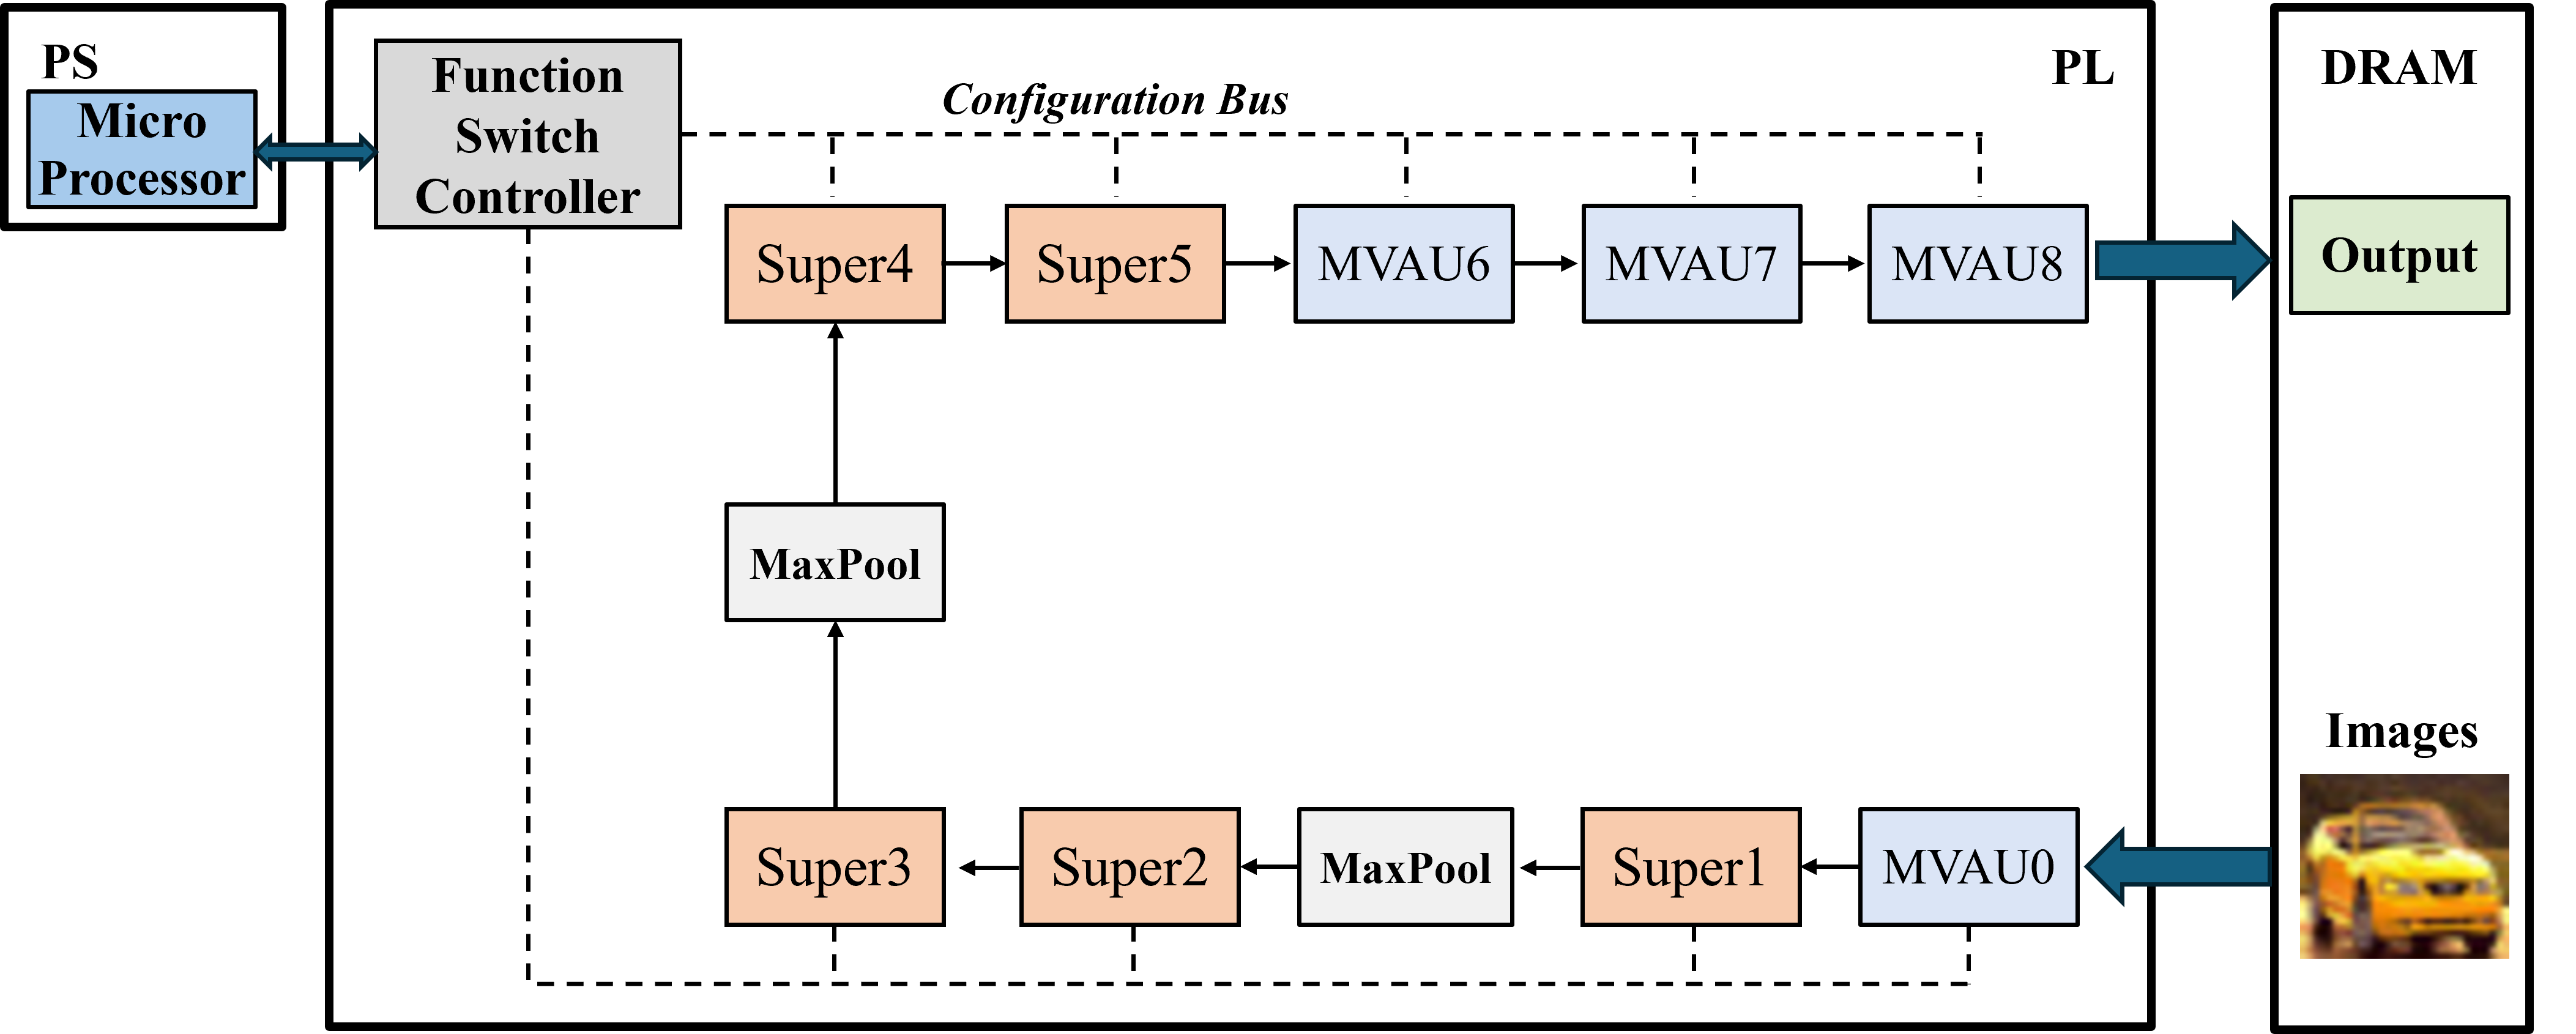
\includegraphics[width=0.78\textwidth]{fig44_mars_arch.png}
\caption{MARS streaming dataflow on the Zynq PL: MVAU0, adapter-enhanced Super1--5, and MVAU6--8, with the Function Switch Controller driving the configuration bus.}
\label{fig:arch}
\end{figure*}

\subsection{Adapter-Enhanced Super Wrapper}
Fig.~\ref{fig:wrapper} shows the Super Wrapper. A splitter duplicates the input stream to (i) a modified FINN MVAU core whose in-module thresholding is decoupled so that the raw 32-bit partial sum is exposed, and (ii) the Adapter IP, whose 8-bit contribution passes through a small synchronisation FIFO. A stream adder fuses the two contributions and applies the Q8 threshold, producing the 1-bit output; binarisation therefore happens \emph{after} the adapter contribution is added, which is what makes a post-accumulator adapter possible in a streaming binarised pipeline. The adapter's weight, RC, and $\alpha$-LUT memories are configuration-writable distributed RAM. Denoting the backbone partial sum by $p_o$ and the up-projection popcount by $q_o$, the fused output bit is
\begin{equation}
\hat{y}_o \;=\; \mathbb{I}\Bigl[\, (p_o \ll 8) \;+\; s_o \cdot \mathrm{LUT}_{\alpha}(q_o) \;\ge\; T^{Q8}_o \Bigr],
\label{eq:fusion}
\end{equation}
where $\mathrm{LUT}_{\alpha}$ is the per-layer Q8 contribution table that absorbs $\alpha$, $s_o$ a per-channel sign, and $T^{Q8}_o$ the BatchNorm-fused threshold in Q8. Everything on the right-hand side is either a shift, a table look-up, or an integer add---no multiplier is instantiated.

\begin{figure}[!t]
\centering
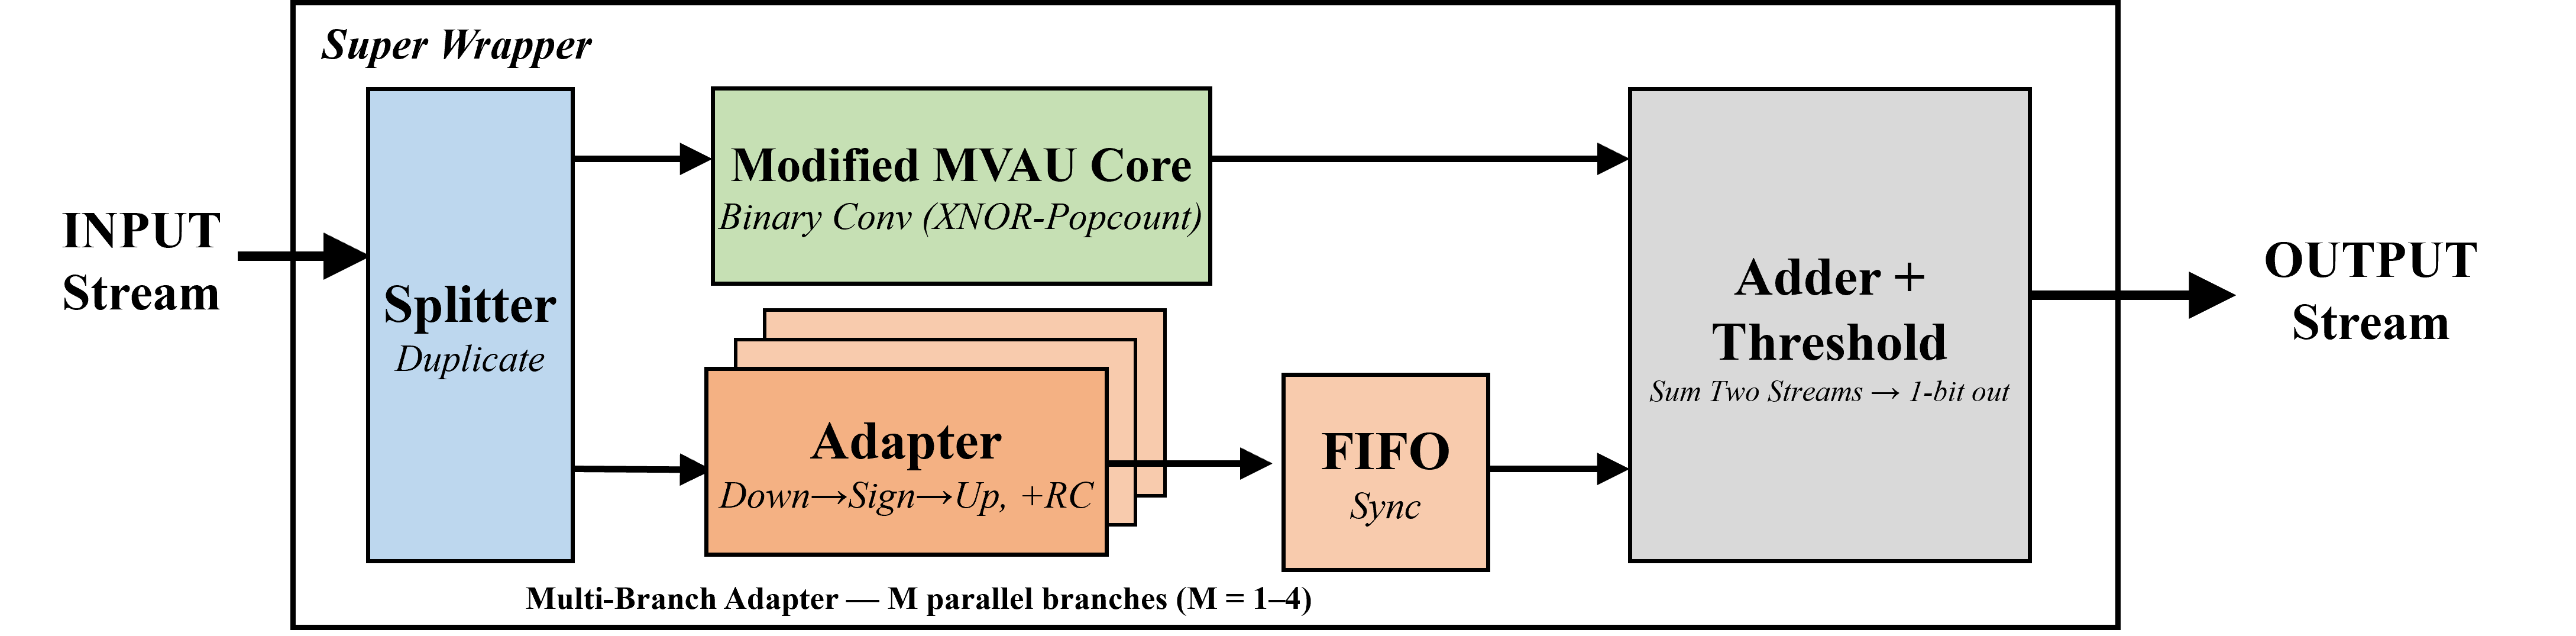
\includegraphics[width=0.92\columnwidth]{hw_super_wrapper.png}
\caption{MVAU + Adapter Super Wrapper: the modified MVAU core exposes raw partial sums; the adapter contribution is fused before the shared Q8 threshold.}
\label{fig:wrapper}
\end{figure}

Fig.~\ref{fig:adapterip} details the Adapter IP datapath: a two-stage pipeline in which the down-projection XNOR--popcount accumulates onto an accumulator whose initial value is the RC bias, the sign stage produces the binary hidden vector, and the up-projection XNOR--popcount feeds a Q8 $\alpha$-LUT that emits the branch contribution. All weight, RC, and LUT memories are configuration-writable distributed RAM fed by the FSC.

\begin{figure}[!t]
\centering
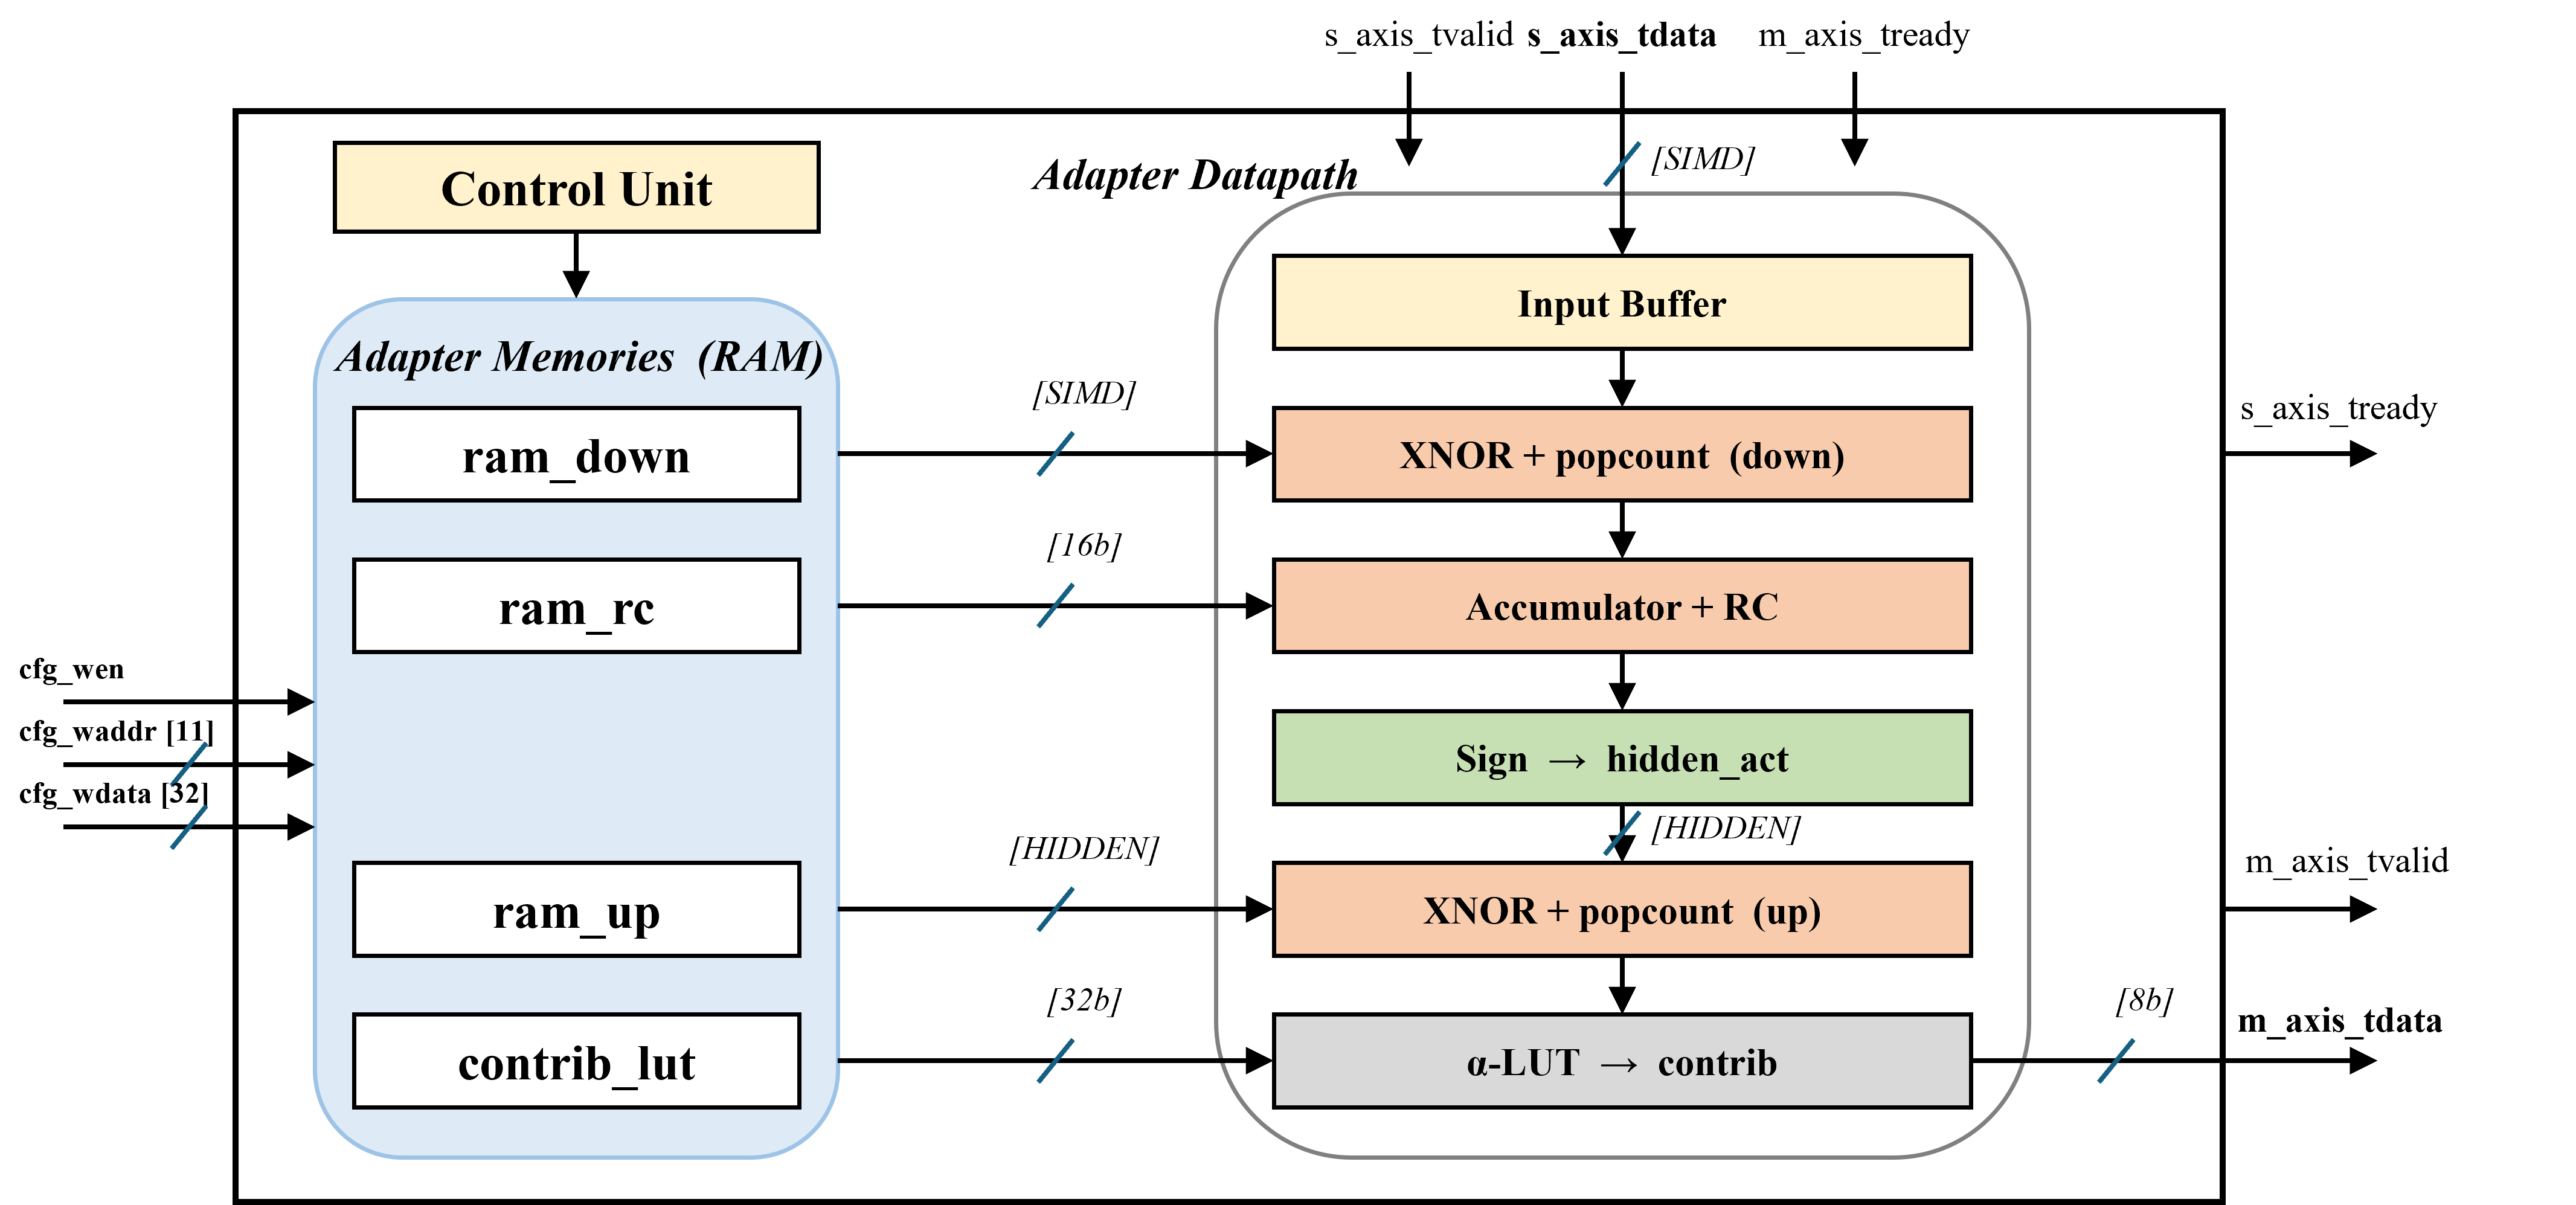
\includegraphics[width=0.92\columnwidth]{hw_adapter_internal.png}
\caption{Adapter IP internal datapath. The RC bias enters as the accumulator initial value; the $\alpha$-LUT converts the up-projection popcount into the Q8 branch contribution.}
\label{fig:adapterip}
\end{figure}

\subsection{Function Switch Controller}
The FSC is an AXI-Lite slave with a 64~KB aperture. A write FSM latches the 16-bit address, decomposes it combinationally into a 3-bit unit select and an 11-bit word address, and issues a single-cycle write-enable pulse to one of nine destinations (MVAU0 thresholds, MVAU8 classifier weights, the five Super adapters, and the MVAU6/MVAU7 thresholds) while broadcasting the shared address/data bus. The entire switching infrastructure costs 19 LUTs, zero BRAM, and zero DSP, and is orthogonal to the streaming datapath: no inference-path logic is touched.

Fig.~\ref{fig:fsc} shows the internal circuit. Table~\ref{tab:map} gives the address map.

\begin{table}[!t]
\centering
\caption{FSC address map (64~KB aperture).}
\label{tab:map}
\small
\setlength{\tabcolsep}{4pt}
\resizebox{\columnwidth}{!}{%
\begin{tabular}{lll}
\toprule
\textbf{Unit} & \textbf{Byte Range} & \textbf{Target} \\
\midrule
0 low  & \texttt{0x0000--0x0FFF} & MVAU0 thresholds (64 w) \\
0 high & \texttt{0x1000--0x1FFF} & MVAU8 classifier weights (1024 w) \\
1--5   & \texttt{0x2000--0xBFFF} & \makecell[l]{Super1--5 adapter: enable, RC,\\down/up weights, thresh, sign, $\alpha$-LUT} \\
6      & \texttt{0xC000--0xDFFF} & MVAU6 thresholds (512 w) \\
7      & \texttt{0xE000--0xFFFF} & MVAU7 thresholds (512 w) \\
\bottomrule
\end{tabular}%
}
\end{table}


\begin{figure*}[!t]
\centering
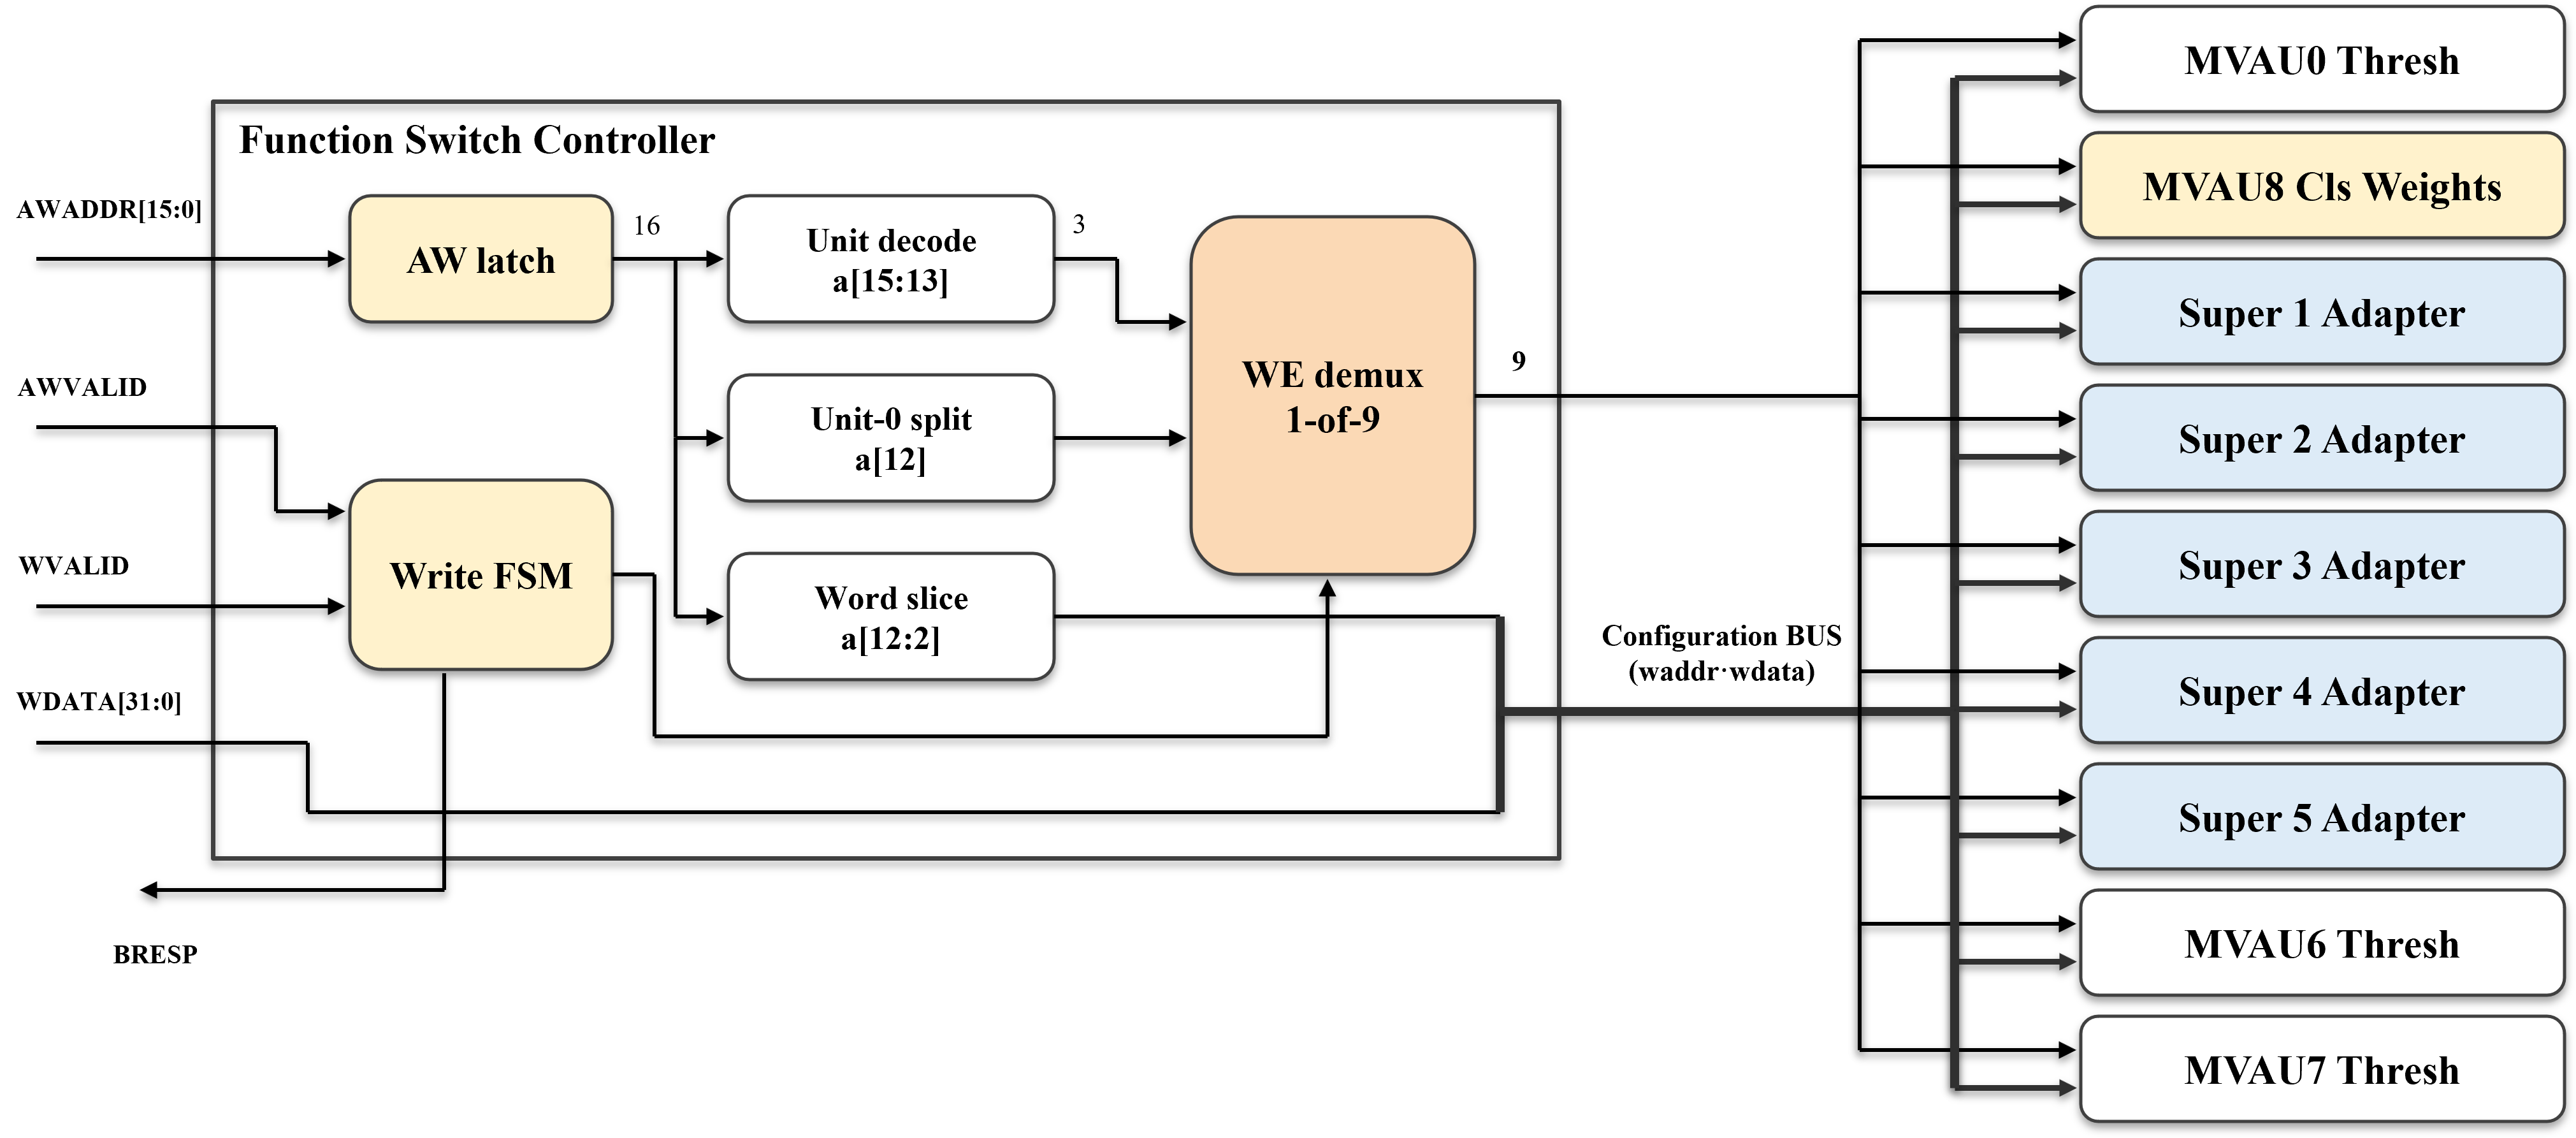
\includegraphics[width=0.66\textwidth]{fsc_circuit.png}
\caption{Function Switch Controller: AW latch, write FSM, combinational address slicing, and a 1-of-9 write-enable demultiplexer over a shared configuration bus.}
\label{fig:fsc}
\end{figure*}

\subsection{Runtime Task Switching}
Because every eligible task shares the same frozen backbone, the binary convolution and FC weights baked into the bitstream are identical across tasks; only the BatchNorm-fused thresholds, the classifier projection, and the adapter parameters differ. A full task switch is therefore a $\approx$25~KB configuration rewrite (25{,}088 stored bytes; 6{,}757 32-bit word writes, i.e.\ 27{,}028 bus bytes, since sub-word fields are widened to full words on the configuration bus), shown in Fig.~\ref{fig:switch}: wait for the output-DMA done flag, bulk-write the new task blob over MMIO, and launch the next batch---no additional flush beyond the output-DMA-done barrier and no fabric reconfiguration. Each additional task costs only an off-line host-side blob; the on-chip cost is $O(1)$ in the task count, bounded by the shared frozen backbone, the $32{\times}32{\times}3$ input format, the shared 10-class output-head interface, and the classification-task assumption.

\begin{figure*}[!t]
\centering
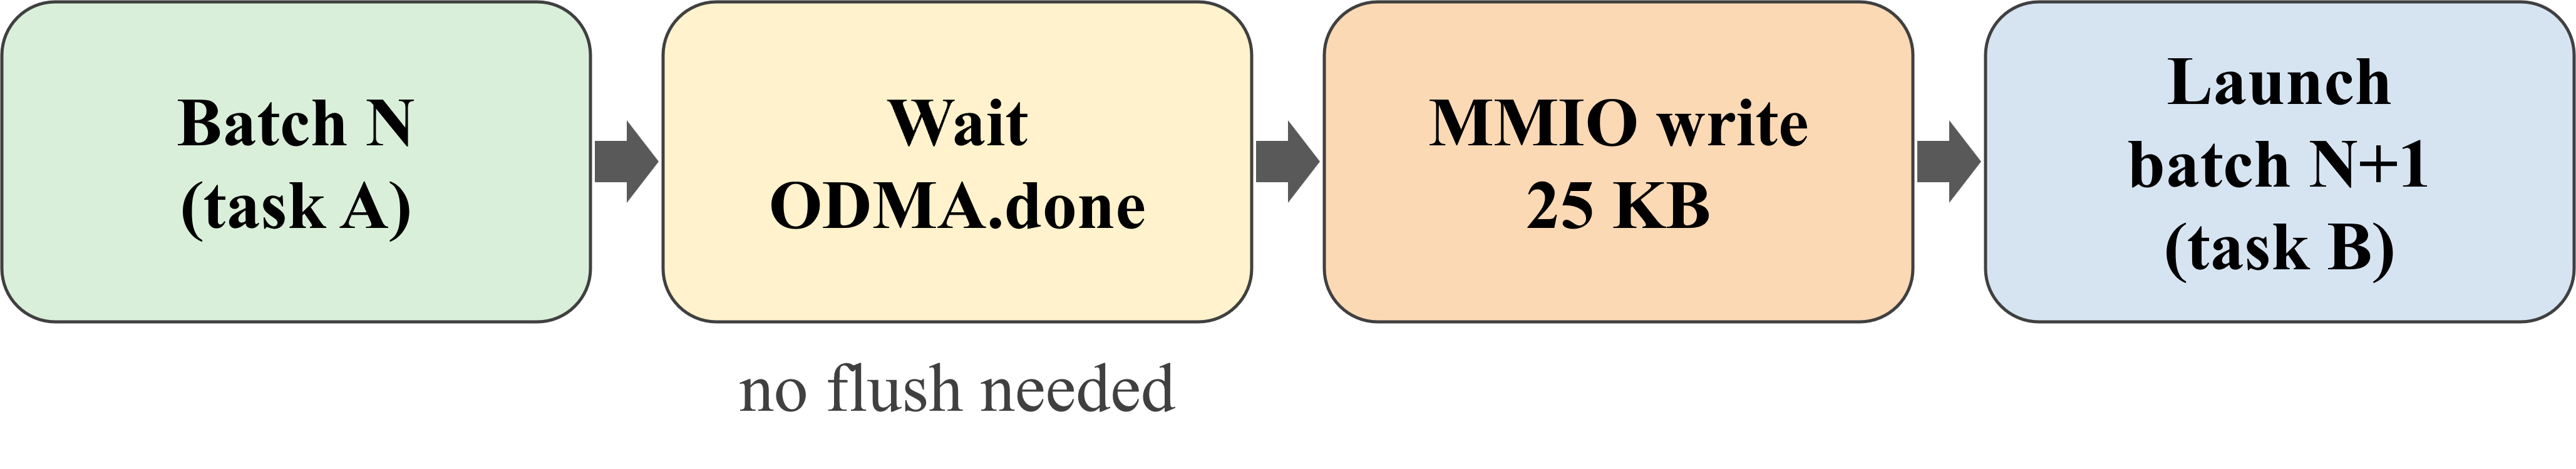
\includegraphics[width=0.62\textwidth]{task_switch.png}
\caption{End-to-end runtime task-switching sequence.}
\label{fig:switch}
\end{figure*}

Two builds of the same architecture are used consistently: a \emph{throughput} build with FINN-default heterogeneous folding (PE up to 32), and a \emph{compactness} build with uniform PE${=}1$ convolutions that trades throughput for the slice headroom hosting fully runtime-writable per-task state. Table~\ref{tab:twovsn} summarises how the two builds realise two depths of the same mechanism. Table~\ref{tab:fold} lists the per-layer folding (visualised in Fig.~\ref{fig:pe_diff}), and Table~\ref{tab:ram} the adapter memories of one representative Super Wrapper; all adapter state is distributed RAM, which is why BRAM does not grow with the adapter.

\begin{table}[!t]
\centering
\caption{Per-layer PE folding of the two builds.}
\label{tab:fold}
\small
\resizebox{\columnwidth}{!}{%
\begin{tabular}{ccc}
\toprule
\textbf{Unit} & \textbf{Throughput PE} & \textbf{Compactness PE} \\
\midrule
MVAU0  & 16 & 1 \\
Super1 & 32 & 1 \\
Super2 & 16 & 1 \\
Super3 & 16 & 1 \\
Super4 & 4  & 1 \\
Super5 & 1  & 1 \\
MVAU6  & 1  & 1 \\
MVAU7  & 1  & 1 \\
MVAU8  & 5  & 5 \\
\bottomrule
\end{tabular}%
}
\end{table}

\begin{figure}[!t]
\centering
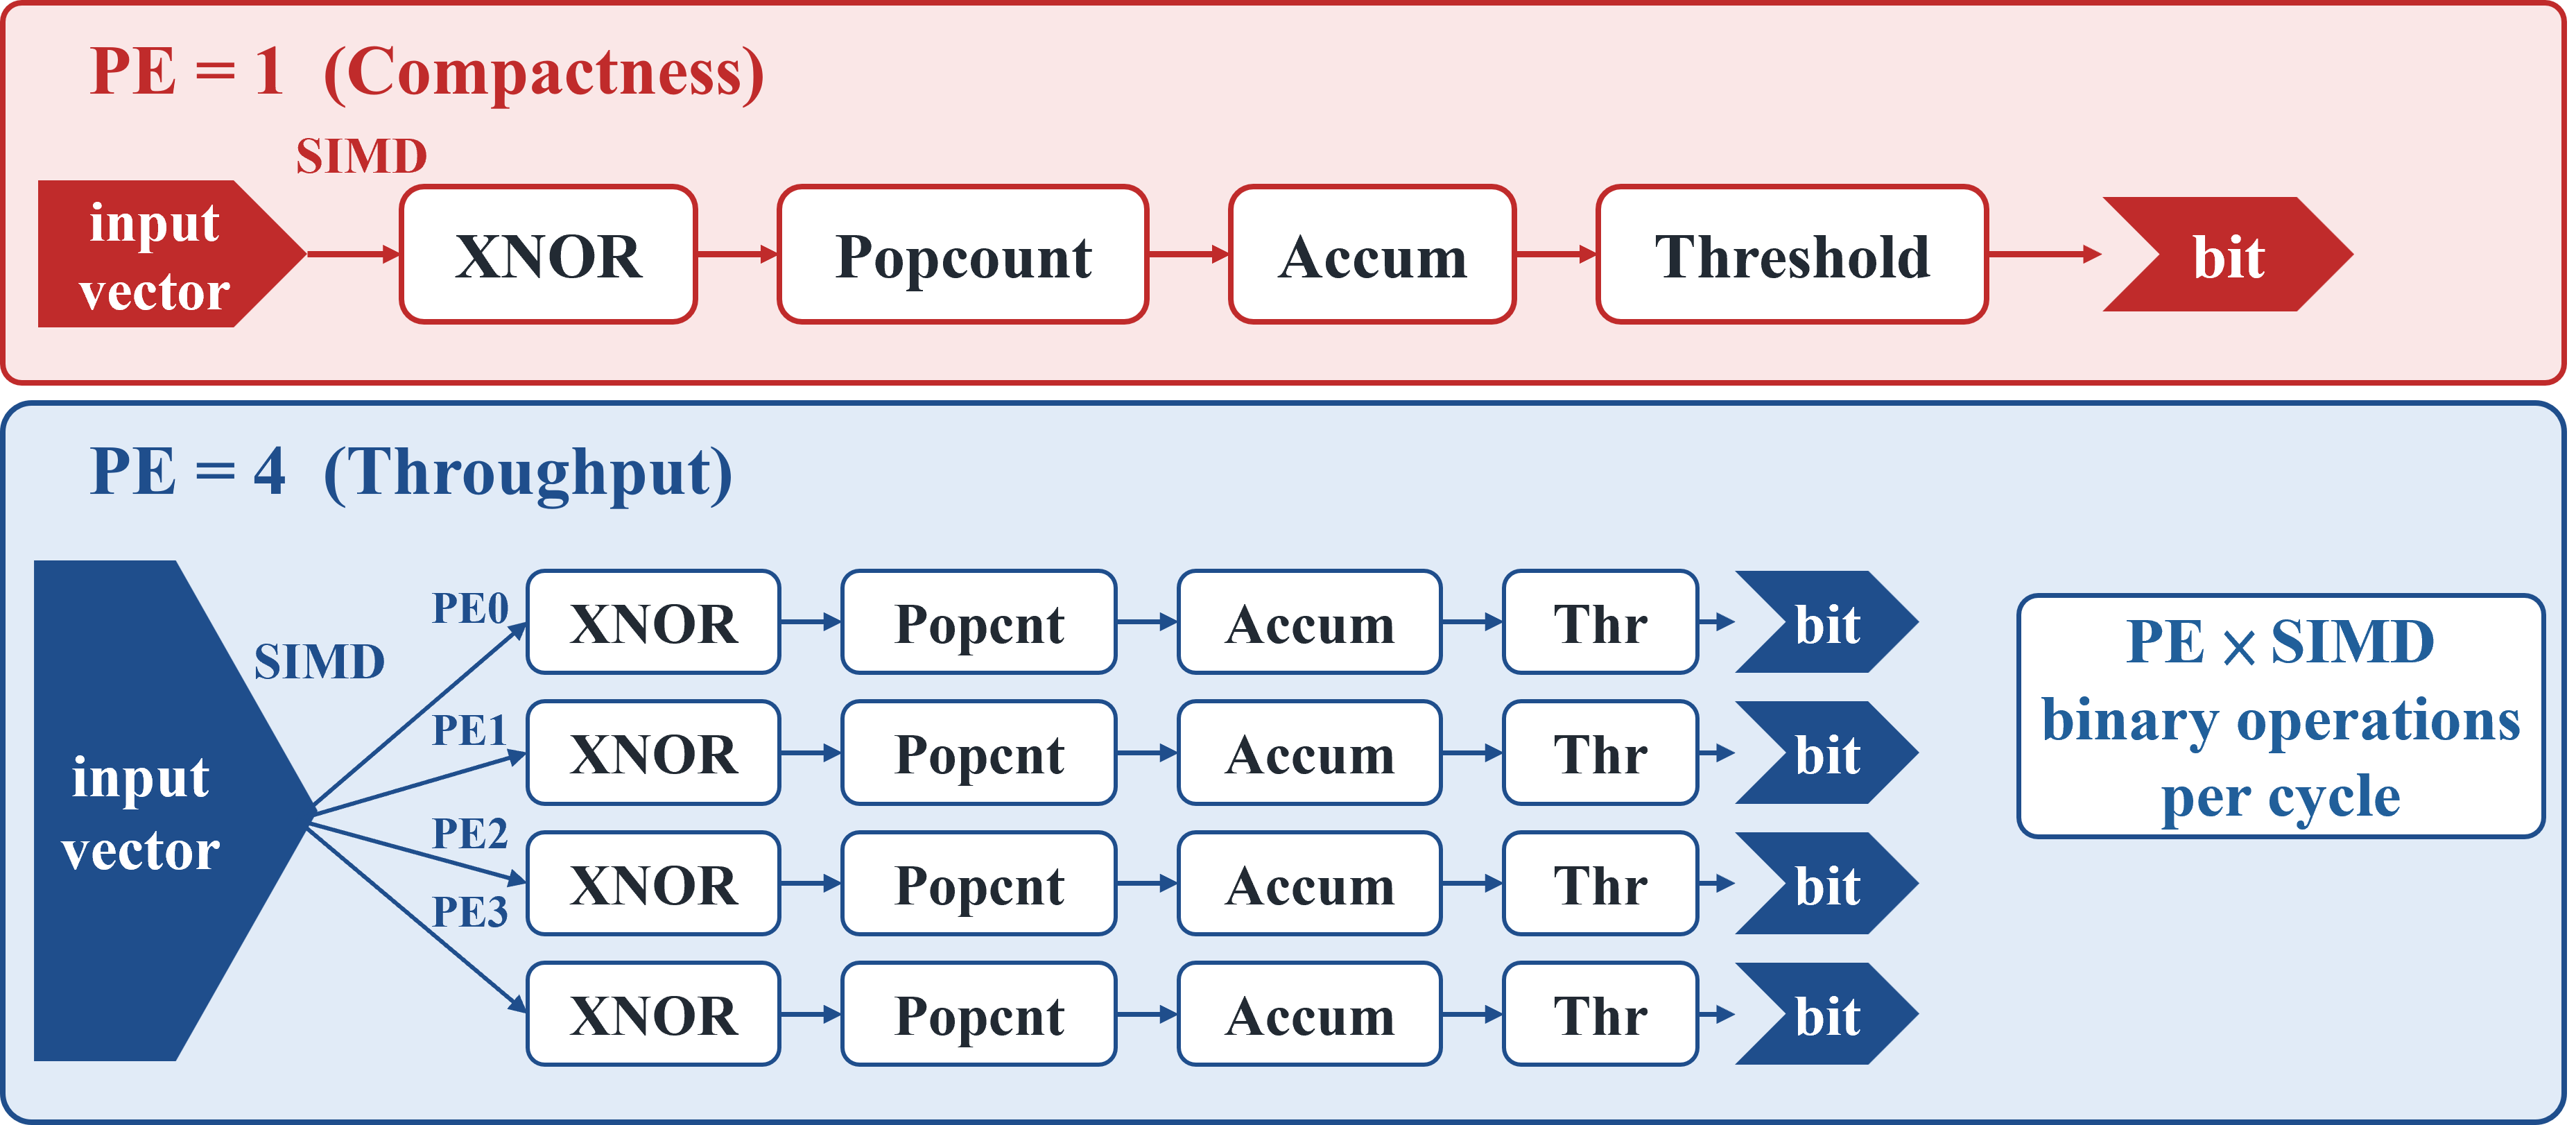
\includegraphics[width=\columnwidth]{pe_diff.png}
\caption{Folding difference between the builds: PE${=}1$ (compactness) vs.\ PE-parallel lanes (throughput, illustrated for PE${=}4$); a unit completes PE$\times$SIMD binary operations per cycle.}
\label{fig:pe_diff}
\end{figure}

\begin{table}[!t]
\centering
\caption{Adapter memories (example: Super4, PE${=}4$).}
\label{tab:ram}
\small
\setlength{\tabcolsep}{3.5pt}
\resizebox{\columnwidth}{!}{%
\begin{tabular}{llll}
\toprule
\textbf{RAM} & \textbf{Depth} & \textbf{Width} & \textbf{Contents} \\
\midrule
\texttt{ram\_down} & 128 & 32~b & down-projection weights \\
\texttt{ram\_up}   & 64  & 128~b & packed up-projection weights \\
\texttt{ram\_rc}   & 32  & 16~b & RC bias (signed) \\
\texttt{contrib\_lut} & 256 & 32~b & Q8 contribution ($\alpha$ absorbed) \\
\bottomrule
\end{tabular}%
}
\end{table}


\begin{table}[!t]
\centering
\caption{Two-task vs.\ $N$-task switching: same mechanism, two depths.}
\label{tab:twovsn}
\small
\setlength{\tabcolsep}{3.5pt}
\resizebox{\columnwidth}{!}{%
\begin{tabular}{lll}
\toprule
 & \textbf{Throughput (2-task)} & \textbf{Compactness ($N$-task)} \\
\midrule
Folding & heterog.\ PE $\le 32$ & uniform PE = 1 \\
Baked at synthesis & one adapter task & nothing (memories empty) \\
Moved per switch & thr.\ + classifier $\approx$15 KB & full blob $\approx$25 KB \\
Reachable models & exactly two & any eligible same-backbone task \\
Verified & on-board, 2 tasks & on-board, 5 tasks \\
\bottomrule
\end{tabular}%
}
\end{table}

\subsection{Design Choices}
Three choices deserve justification. \emph{Distributed RAM over BRAM:} adapter memories are small, wide, and read every cycle; LUT-RAM keeps them adjacent to their datapaths and leaves the BRAM budget to the backbone memstreams, which is why the adapter adds zero BRAM. \emph{Splitter + FIFO synchronisation:} the adapter side-stream must rejoin the folded MVAU stream cycle-accurately under backpressure; a small synchronisation FIFO absorbs the latency skew so that the fused threshold sees matched operands, which is what keeps adapter-enabled throughput within $\approx$0.5\% of the backbone. \emph{Q8 fixed point:} the selected eight-fractional-bit format keeps the measured software-to-board gap below one percentage point in the deployed experiments (Table~\ref{tab:onboard}); a systematic precision sweep of this scaling was not performed.

\section{Experimental Results}
\subsection{Setup}
Software experiments use PyTorch with Brevitas~\cite{Pappalardo2021Brevitas} quantisation-aware training (200 epochs, ADAM, lr 0.005, step decay, seed 2024); hardware is generated through FINN and Vivado 2022.2 and deployed on a PYNQ-Z2 (XC7Z020). Five $32{\times}32{\times}3$ classification datasets are used: CIFAR-10 (backbone source), SVHN, FashionMNIST, STL10, and CINIC10. Functional correctness is established at three levels: per-module RTL simulation (43{,}520 vectors, 100\% pass), top-level dataflow simulation against the PyTorch golden model, and end-to-end on-board execution.

Table~\ref{tab:data} lists the five datasets; all are adapted to the backbone's $32{\times}32{\times}3$ input (STL10 downscaled, FashionMNIST resized and channel-replicated). For each transfer, the backbone is frozen and the adapter and classifier are trained for 200 epochs with SqrHinge loss. Following the original BNN-PYNQ trainer flow, the best epoch is selected by test-set accuracy (no held-out validation split), so absolute accuracies are best-of-200-epoch operating points and may be optimistically biased; every configuration uses the identical rule, making comparisons procedurally consistent, although best-epoch selection on the test split may also bias relative differences.

\begin{table}[!t]
\centering
\caption{Datasets (all adapted to a $32{\times}32{\times}3$ input).}
\label{tab:data}
\small
\setlength{\tabcolsep}{3.5pt}
\resizebox{\columnwidth}{!}{%
\begin{tabular}{lccl}
\toprule
\textbf{Dataset} & \textbf{Classes} & \textbf{Train / Test} & \textbf{Notes} \\
\midrule
CIFAR-10     & 10 & 50{,}000 / 10{,}000 & natural objects (backbone) \\
SVHN         & 10 & 73{,}257 / 26{,}032 & house-number digits \\
STL10        & 10 & 5{,}000 / 8{,}000   & ImageNet-derived, $96^2$ native \\
FashionMNIST & 10 & 60{,}000 / 10{,}000 & clothing, grayscale \\
CINIC10      & 10 & 90{,}000 / 90{,}000 & CIFAR + ImageNet mix \\
\bottomrule
\end{tabular}%
}
\end{table}

\subsection{Three-Level Functional Verification}
Correctness is established bottom-up. (i) \emph{Module level:} each Super Wrapper is simulated standalone against a memblock-faithful golden model---43{,}520 output vectors across the five adapter-hosting layers, 100\% bit-exact. (ii) \emph{Top level:} the complete stitched pipeline (DMA, MVAU0, Super1--5, pooling, MVAU6--8, label select) is simulated as one block design against the PyTorch reference. (iii) \emph{Board level:} the generated bitstream executes the full test sets end-to-end. One methodological note: when RTL sources inside a stitched IP change, Vivado's per-IP out-of-context synthesis cache must be reset explicitly, otherwise a stale netlist silently masks configuration writes---a failure mode worth documenting for reproducibility.

\subsection{Residual Correction at 1 Bit}
Table~\ref{tab:rc} isolates RC on CIFAR-10$\to$SVHN in the wide software geometry. RC contributes $+15$ to $+17$~pp at every branch count, and $+23.0$~pp in the deployed ($1{\times}1$, scalar-$\alpha$) geometry; at ${\geq}2$-bit precision the same term shifts accuracy typically within $\pm 0.3$~pp (maximum observed $1.4$~pp), demonstrating a substantially larger effect at 1W1A in the evaluated sweep. On the other transfer targets, RC gains range from $+0.6$ to $+7.4$~pp.

\begin{table}[!t]
\centering
\caption{RC ablation at 1 bit, wide geometry (CIFAR-10 $\to$ SVHN).}
\label{tab:rc}
\small
\resizebox{\columnwidth}{!}{%
\begin{tabular}{llrrrr}
\toprule
\textbf{Adapter} & \textbf{M} & \textbf{No-RC} & \textbf{With RC} & \textbf{$\Delta_{\text{RC}}$} & \textbf{Full-FT} \\
\midrule
Conv-Adapter~\cite{Chen2024ConvAdapter} & 1 & 63.06\% & 79.23\% & +16.17 & \multirow{4}{*}{94.91\%} \\
\cmidrule(lr){1-5}
\multirow{3}{*}{\textbf{MARS}} & 2 & 66.12\% & 83.01\% & +16.89 & \\
 & 3 & 67.79\% & 83.48\% & +15.69 & \\
 & 4 & 69.08\% & \textbf{84.44\%} & +15.36 & \\
\bottomrule
\end{tabular}%
}
\end{table}

\subsection{Multi-Branch Scaling in Software}
Table~\ref{tab:mbsw} reports the wide-geometry software branch sweep on the CIFAR-10 backbone, with the largest gains on hard transfers and diminishing returns as $M$ grows. The headline numbers come from the \emph{deployed-geometry} sweep over all twenty backbone--target pairs spanning five source backbones (Table~\ref{tab:mbdep}): multi-branch scaling improves 1-bit transfer accuracy by $+3.36$~pp on average over the single-branch Conv-Adapter baseline, up to $+11.33$~pp (FashionMNIST$\to$SVHN).

\begin{table}[!t]
\centering
\caption{Multi-branch scaling on the CIFAR-10 backbone (wide geometry, software, 1W1A, RC).}
\label{tab:mbsw}
\small
\setlength{\tabcolsep}{3.5pt}
\resizebox{\columnwidth}{!}{%
\begin{tabular}{lccccc}
\toprule
 & \textbf{\cite{Chen2024ConvAdapter}} & \multicolumn{3}{c}{\textbf{MARS}} & \\
\cmidrule(lr){2-2}\cmidrule(lr){3-5}
\textbf{Target} & \textbf{$M{=}1$} & \textbf{$M{=}2$} & \textbf{$M{=}3$} & \textbf{$M{=}4$} & \textbf{Full-FT} \\
\midrule
SVHN         & 79.23 & 83.01 & 83.48 & \textbf{84.44} & 94.91 \\
STL10        & 67.50 & 67.48 & 67.68 & \textbf{68.15} & 71.05 \\
FashionMNIST & 82.71 & 83.57 & \textbf{83.63} & 83.60 & 92.36 \\
CINIC10      & 64.50 & 64.71 & 64.85 & \textbf{65.02} & 68.02 \\
\bottomrule
\end{tabular}%
}
\end{table}

Table~\ref{tab:backbones} extends the wide-geometry software study to the remaining sixteen pairs across the four additional source backbones, with gains up to $+7.63$~pp (STL10$\to$SVHN). In the deployed-geometry sweep of Table~\ref{tab:mbdep}, every one of the twenty pairs improves, up to $+11.33$~pp on FashionMNIST$\to$SVHN. Five-seed paired checks on two deployment-relevant transfers provide preliminary evidence of a positive $M{=}1{\to}4$ gain under the same test-selected checkpoint protocol: $+6.64 \pm 0.43$~pp on SVHN (95\% CI $[+6.10, +7.18]$) and $+2.69 \pm 0.36$~pp on FashionMNIST (95\% CI $[+2.25, +3.13]$); a selection-free final-epoch reading of the same training logs yields consistent paired gains ($+6.87 \pm 0.50$ and $+2.99 \pm 0.40$~pp). On the CIFAR-10 deployment backbone the deployed ($1{\times}1$, scalar-$\alpha$) geometry preserves the broad target-wise trend of the wide geometry; elsewhere the ranking is source-dependent, and under severe mismatch the deployed geometry can exceed the wide one. All hardware results below use the deployed geometry.

\begin{table*}[!t]
\centering
\caption{Multi-branch adapter scaling across other source backbones (wide geometry, 1W1A, RC).}
\label{tab:backbones}
\small
\setlength{\tabcolsep}{4pt}
\resizebox{\textwidth}{!}{%
\begin{tabular}{llcccccc}
\toprule
 & & \textbf{Conv-Adapter}~\cite{Chen2024ConvAdapter} & \multicolumn{3}{c}{\textbf{MARS}} & & \\
\cmidrule(lr){3-3}\cmidrule(lr){4-6}
\textbf{Backbone} & \textbf{Target} & \textbf{$M{=}1$} & \textbf{$M{=}2$} & \textbf{$M{=}3$} & \textbf{$M{=}4$} & \textbf{$\Delta_{\text{multi}}$ (pp)} & \textbf{Full-FT} \\
\midrule
SVHN & CIFAR-10     & 46.34 & 49.54 & 49.56 & \textbf{50.41} & +4.07 & 81.70 \\
SVHN & STL10        & 35.16 & 37.48 & 37.60 & \textbf{38.46} & +3.30 & 63.14 \\
SVHN & FashionMNIST & 81.47 & 82.40 & 82.86 & \textbf{83.02} & +1.55 & 92.32 \\
SVHN & CINIC10      & 32.76 & 34.47 & 36.84 & \textbf{39.70} & +6.94 & 67.85 \\
\midrule
STL10 & CIFAR-10     & 68.92 & 69.97 & 70.58 & \textbf{70.99} & +2.07 & 83.01 \\
STL10 & FashionMNIST & 84.71 & 85.77 & 86.28 & \textbf{86.35} & +1.64 & 92.73 \\
STL10 & SVHN         & 73.22 & 77.53 & 80.16 & \textbf{80.85} & +7.63 & 95.32 \\
STL10 & CINIC10      & 56.07 & 56.74 & \textbf{57.39} & 57.36 & +1.29 & 70.18 \\
\midrule
FashionMNIST & CIFAR-10 & 30.42 & 30.54 & 32.64 & \textbf{33.26} & +2.84 & 78.37 \\
FashionMNIST & STL10    & 30.84 & 31.94 & \textbf{33.20} & 31.81 & +0.97 & 59.11 \\
FashionMNIST & SVHN     & 39.16 & 43.29 & 45.68 & \textbf{45.68} & +6.52 & 94.36 \\
FashionMNIST & CINIC10  & 24.82 & 25.33 & \textbf{27.28} & 26.34 & +1.52 & 64.63 \\
\midrule
CINIC10 & CIFAR-10     & 78.05 & 78.08 & 78.47 & \textbf{78.59} & +0.54 & 80.92 \\
CINIC10 & SVHN         & 67.43 & 70.60 & 71.12 & \textbf{72.30} & +4.87 & 94.62 \\
CINIC10 & STL10        & 66.42 & 66.86 & 67.33 & \textbf{67.83} & +1.41 & 70.38 \\
CINIC10 & FashionMNIST & 79.81 & 80.89 & 81.26 & \textbf{81.59} & +1.78 & 91.99 \\
\bottomrule
\end{tabular}%
}
\end{table*}

\subsection{Resource, Power, and Branch Cost}
Table~\ref{tab:resource} compares four post-implementation builds on the XC7Z020. Integrating the adapter and the switching infrastructure raises the throughput build to $78.4\%$ LUTs at $99.8\%$ slice occupancy; the deployed compactness build reaches $75.1\%$ LUTs while providing the runtime-writable state for one active task; the five task images reside on the host and are loaded in turn. All builds use zero DSPs, and the adapter does not increase BRAM: all adapter memories live in distributed RAM. On-chip power (Vivado post-route estimate) is 2.215~W for the adapter-enabled throughput build ($+0.101$~W over its backbone) and 1.802~W for the compactness build. Post-route hierarchical analysis attributes roughly 25{,}593 LUTs ($\approx$48\% of the chip) to the five adapter-hosting Super Wrappers, dominated by the adapter weight RAMs, XNOR--popcount trees, and threshold comparators, consistent with MVAU resource-prediction studies~\cite{Arend2025MVAUPredict}; occupied-slice utilisation ($97$--$100\%$) saturates before LUT utilisation because control-set constraints spread the design across the placement grid. Table~\ref{tab:cost} quantifies the linear per-branch cost; $M{\geq}2$ exceeds the XC7Z020 post-synthesis and is verified at the RTL-simulation and post-synthesis levels only (not placed-and-routed or on-board), and Fig.~\ref{fig:tradeoff} plots the resulting accuracy-versus-LUT trade-off.

On the throughput build, integrating the adapter and the switching infrastructure raises total on-chip power by only $+0.101$~W ($+4.8\%$, $2.114 \to 2.215$~W), the dynamic term rising from $1.949$ to $2.046$~W; the FSC itself adds negligible power. (The $2.215$~W build includes the FSC; the cross-platform comparison of Table~\ref{tab:xplat} uses the $2.214$~W adapter-enabled throughput build without it.) The compactness build sits lower ($1.78$--$1.80$~W) because uniform PE${=}1$ folding instantiates far less parallel logic. The $\approx$$17.4\times$ throughput difference between the builds ($107 \to 1{,}859$~img/s on the backbone) is the price of the folding design point, not an optimisation introduced here; the pipelining contribution of this work is that adapter-enabled throughput stays within $\approx$0.5\% of the corresponding backbone, because the adapter side-stream is cycle-accurately synchronised into the folded datapath.

\begin{table*}[!t]
\centering
\caption{FPGA resource utilisation across four MARS build configurations (post-implementation, XC7Z020).}
\label{tab:resource}
\small
\resizebox{\textwidth}{!}{%
\begin{tabular}{lcrrrr}
\toprule
\textbf{Configuration} & \textbf{Function Switch} & \textbf{Occupied Slices} & \textbf{Slice LUTs} & \textbf{Slice Reg.\ (FF)} & \textbf{BRAM} \\
\midrule
Backbone (Throughput)      & no  & 11{,}648 (87.58\%) & 25{,}322 (47.60\%) & 31{,}621 (29.72\%) & 99.5 (71.07\%) \\
MARS (Throughput, 2-task)  & yes & 13{,}272 (99.79\%) & 41{,}729 (78.44\%) & 53{,}285 (50.08\%) & 99 (70.71\%) \\
Backbone (Compactness)     & no  & 8{,}926 (67.11\%)  & 15{,}651 (29.42\%) & 22{,}219 (20.88\%) & 85 (60.71\%) \\
MARS (Compactness, N-task) & yes & 12{,}957 (97.42\%) & 39{,}967 (75.13\%) & 40{,}926 (38.46\%) & 84 (60.00\%) \\
\bottomrule
\end{tabular}%
}
\end{table*}

\begin{table}[!t]
\centering
\caption{Per-branch parameter and post-synthesis cost (compactness build).}
\label{tab:cost}
\small
\setlength{\tabcolsep}{3.5pt}
\resizebox{\columnwidth}{!}{%
\begin{tabular}{ccccc}
\toprule
\textbf{M} & \textbf{Params} & \textbf{vs.\ Backbone} & \textbf{Slice LUTs (\%)} & \textbf{Power (W)} \\
\midrule
1 & 58{,}533  & $+3.78\%$  & 47{,}931 (90.1\%)   & 1.841 \\
2 & 117{,}066 & $+7.57\%$  & 71{,}841 (135.0\%)  & 1.897 \\
3 & 175{,}599 & $+11.35\%$ & 95{,}593 (179.7\%)  & 1.915 \\
4 & 234{,}132 & $+15.14\%$ & 125{,}538 (236.0\%) & 1.969 \\
\bottomrule
\end{tabular}%
}
\end{table}

\begin{table}[!t]
\centering
\caption{Deployed-geometry multi-branch transfer accuracy (\%) over all twenty backbone--target pairs ($M{=}1$--$4$, RC on; single seed). $\Delta_{\text{multi}} = M{=}4 - M{=}1$ (pp).}
\label{tab:mbdep}
\small
\setlength{\tabcolsep}{3pt}
\resizebox{\columnwidth}{!}{%
\begin{tabular}{llccccc}
\toprule
\textbf{Backbone} & \textbf{Target} & $M{=}1$ & $M{=}2$ & $M{=}3$ & $M{=}4$ & $\Delta_{\text{multi}}$ \\
\midrule
CIFAR-10 & SVHN & 73.72 & 77.16 & 78.77 & 79.81 & $+6.09$ \\
 & FashionMNIST & 80.42 & 82.00 & 82.82 & 83.54 & $+3.12$ \\
 & STL10 & 67.46 & 67.58 & 68.00 & 68.06 & $+0.60$ \\
 & CINIC10 & 64.80 & 65.16 & 65.38 & 65.45 & $+0.65$ \\
SVHN & CIFAR-10 & 43.18 & 45.13 & 46.93 & 48.37 & $+5.19$ \\
 & FashionMNIST & 78.51 & 79.76 & 80.56 & 81.89 & $+3.38$ \\
 & STL10 & 34.41 & 34.60 & 35.45 & 35.10 & $+0.69$ \\
 & CINIC10 & 33.59 & 35.21 & 34.29 & 38.03 & $+4.44$ \\
STL10 & CIFAR-10 & 66.65 & 67.90 & 68.74 & 68.79 & $+2.14$ \\
 & FashionMNIST & 81.48 & 82.96 & 83.58 & 84.19 & $+2.71$ \\
 & SVHN & 68.15 & 73.18 & 74.17 & 75.65 & $+7.50$ \\
 & CINIC10 & 54.26 & 55.33 & 56.17 & 56.56 & $+2.30$ \\
FashionMNIST & CIFAR-10 & 33.63 & 34.67 & 35.84 & 36.76 & $+3.13$ \\
 & STL10 & 32.64 & 32.29 & 33.64 & 34.11 & $+1.47$ \\
 & SVHN & 51.37 & 58.19 & 59.42 & 62.70 & $+11.33$ \\
 & CINIC10 & 27.75 & 28.37 & 29.55 & 29.56 & $+1.81$ \\
CINIC10 & CIFAR-10 & 78.21 & 78.60 & 78.87 & 78.72 & $+0.51$ \\
 & SVHN & 69.14 & 73.88 & 75.39 & 76.34 & $+7.20$ \\
 & STL10 & 67.21 & 67.60 & 67.54 & 67.42 & $+0.21$ \\
 & FashionMNIST & 80.23 & 81.86 & 82.17 & 82.88 & $+2.65$ \\
\midrule
\multicolumn{2}{l}{Mean gain over $M{=}1$ (pp)} & --- & $+1.73$ & $+2.52$ & $+3.36$ & --- \\
\bottomrule
\end{tabular}%
}
\end{table}

\begin{figure}[!t]
\centering
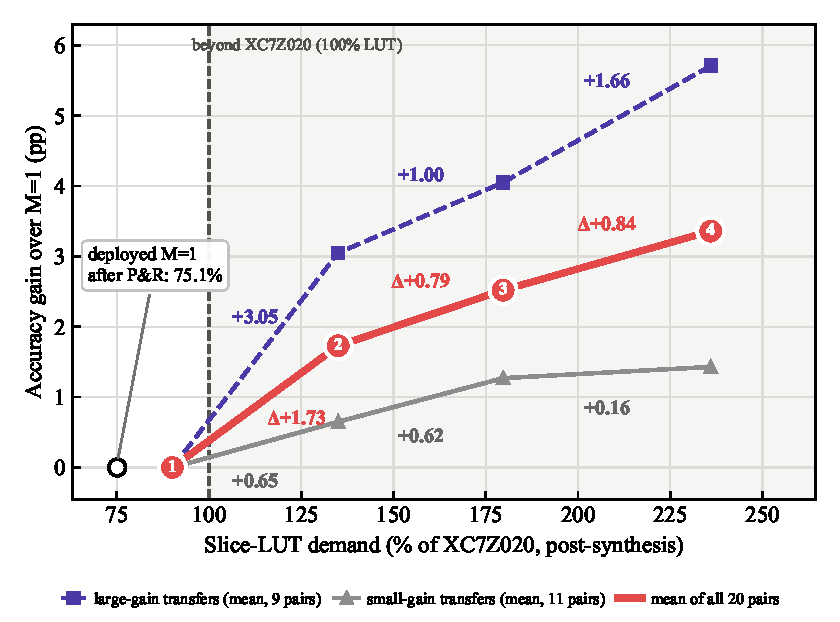
\includegraphics[width=\columnwidth]{mb_tradeoff_compact_lut.pdf}
\caption{Accuracy gain vs.\ post-synthesis LUT demand for multi-branch scaling (compactness build). Large-gain: $\Delta_{\text{multi}} \geq 3$~pp (9 pairs); the remaining 11 pairs form the small-gain group. $M{\geq}2$ exceeds the XC7Z020.}
\label{fig:tradeoff}
\end{figure}

Fig.~\ref{fig:layout} shows the post-implementation placement of the compactness build: adapter logic and backbone MVAUs dominate and interleave across the die, while the Function Switch Controller appears only as a negligible scattering of cells, matching its 19-LUT footprint.

\begin{figure}[!t]
\centering
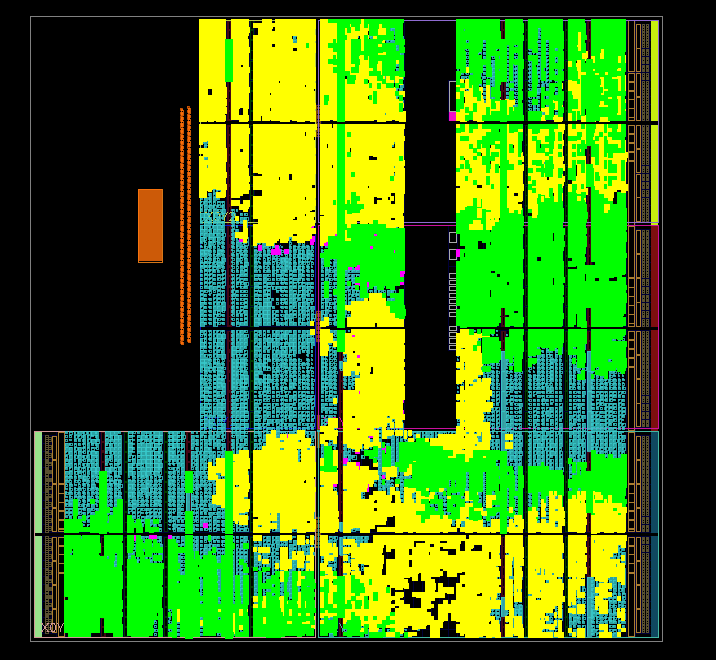
\includegraphics[width=0.72\columnwidth]{mars_soc_layout.png}
\caption{Post-implementation layout of the MARS compactness build on XC7Z020. Yellow: adapter datapaths and adapter RAMs; green: MVAUs; purple: Function Switch Controller; orange: PS; blue: other SoC-integration logic.}
\label{fig:layout}
\end{figure}

\subsection{On-Board Runtime Task Switching}
Table~\ref{tab:onboard} reports on-board accuracy for the five task-specific models served from the single compactness bitstream (loaded in turn from host-resident images), each measured over its 10{,}000-image test set (STL10 over its full 8{,}000). Every task reproduces its software reference within $0.69$~pp; the residual gap is consistent with accumulated fixed-point and threshold-quantisation effects rather than an observed RTL mismatch. Each accuracy figure is the mean of ten runs at batch 1000 over the full test set; the on-board digits are stable across runs. Per-module RTL simulation is bit-exact, so no RTL mismatch was observed; the residual gaps are consistent with Q8 threshold rounding reclassifying a few borderline images. Fifty random task switches yield a configuration-rewrite time of $1.86\pm0.04$~ms (post-switch inference correctness verified separately), dominated by the single-beat AXI-Lite write path. Table~\ref{tab:prior} positions MARS against published task-switching FPGA inference: MARS is the only surveyed system that needs no fabric-PR controller while keeping the task set open after synthesis.

\begin{table}[!t]
\centering
\caption{Compactness build: on-board $N$-task switching accuracy.}
\label{tab:onboard}
\small
\resizebox{\columnwidth}{!}{%
\begin{tabular}{llrrr}
\toprule
\textbf{Dataset} & \textbf{Mode} & \textbf{Software Reference} & \textbf{On-Board} & \textbf{Gap (pp)} \\
\midrule
CIFAR-10     & backbone only & 81.46\% & 80.99\% & $-0.47$ \\
SVHN         & MARS          & 73.72\% & 73.21\% & $-0.51$ \\
FashionMNIST & MARS          & 80.42\% & 79.98\% & $-0.44$ \\
STL10        & MARS          & 67.46\% & 66.77\% & $-0.69$ \\
CINIC10      & MARS          & 64.80\% & 64.64\% & $-0.16$ \\
\bottomrule
\end{tabular}%
}
\end{table}

\begin{table*}[!t]
\centering
\caption{Task-switching FPGA inference: MARS vs.\ published approaches.}
\label{tab:prior}
\small
\resizebox{\textwidth}{!}{%
\begin{tabular}{lcrccl}
\toprule
\textbf{Approach} & \textbf{Year} & \makecell{\textbf{Switch}\\\textbf{Latency}} & \makecell{\textbf{Fabric-PR}\\\textbf{Controller}} & \textbf{Task Storage Scaling} & \textbf{Adaptation Level} \\
\midrule
ACNNE~\cite{Huang2024ACNNE}                      & 2024 & 97--114~ms & Yes (PCAP)  & partial bitstream per task & layer-block swap \\
CoarseToFine~\cite{Rangsikunpum2024CoarseToFine} & 2024 & 5.2~ms     & Yes (ZyCAP) & partial bitstream per task & model-level swap \\
Boudjadar et~al.~\cite{Boudjadar2025DynamicFPGA} & 2025 & PR-bound   & Yes (DPR)   & partial bitstream per task & model-level swap \\
Kang \& Park~\cite{Kang2025RuntimeRobust}        & 2025 & PR-bound   & Yes (DPR)   & partial-update masks per task & partial model update \\
FixyNN~\cite{Whatmough2019FixyNN}                & 2019 & N/A (fixed FE) & No      & back-end hardware per task & fixed FE; per-task back-end \\
NeuroAdaptiveNet~\cite{ElBouazzaoui2025NeuroAdaptive} & 2025 & 0.23--0.67~$\mu$s & No & all variants on-chip (fixed at synthesis) & model/variant select \\
\midrule
\textbf{MARS} & \textbf{2026} & \textbf{1.86~ms} & \textbf{No} & \textbf{$O(1)$ on-chip; $\approx$25~KB host blob/task} & \textbf{FE-level adapters} \\
\bottomrule
\end{tabular}%
}
\end{table*}

Table~\ref{tab:scaling} reports the post-synthesis scaling of both builds for $M{=}1$--$4$: growth is linear and predictable in LUT/FF with BRAM constant and zero DSPs throughout, because every added branch lives entirely in logic and distributed RAM. Synthesis-stage figures overstate the final cost---after place-and-route the deployed $M{=}1$ builds settle at $78.4\%$ (throughput) and $75.1\%$ (compactness) of the device LUTs.

The $1.86$~ms switch amortises to $\approx$0.02\% of a batch-1000 run, and the write path sustains one word per $\approx$275~ns. Storage also scales favourably: serving $T$ tasks requires one full bitstream plus $T$ host-side 25~KB blobs, versus $T$ partial bitstreams (each orders of magnitude larger) for PR-based systems, and versus synthesis-time-fixed on-chip variants for parameter-selection designs.

\begin{table*}[!t]
\centering
\caption{Post-synthesis resource and power scaling of multi-branch MARS on XC7Z020 (BRAM constant, zero DSP).}
\label{tab:scaling}
\small
\resizebox{\textwidth}{!}{%
\begin{tabular}{clrrcc}
\toprule
\textbf{Build} & $M$ & \textbf{Slice LUTs} & \textbf{Slice Reg.\ (FF)} & \textbf{BRAM} & \textbf{Power (W)} \\
\midrule
\multirow{4}{*}{Throughput (2-task)}
 & 1 & 73{,}169 (137.5\%)  & 65{,}717 (61.8\%)   & 99 & 2.135 \\
 & 2 & 109{,}731 (206.3\%) & 86{,}727 (81.5\%)   & 99 & 2.193 \\
 & 3 & 145{,}061 (272.7\%) & 107{,}471 (101.0\%) & 99 & 2.337 \\
 & 4 & 187{,}521 (352.5\%) & 128{,}698 (121.0\%) & 99 & 2.468 \\
\midrule
\multirow{4}{*}{Compactness (N-task)}
 & 1 & 47{,}931 (90.1\%)   & 42{,}922 (40.3\%)   & 84 & 1.841 \\
 & 2 & 71{,}841 (135.0\%)  & 60{,}390 (56.8\%)   & 84 & 1.897 \\
 & 3 & 95{,}593 (179.7\%)  & 77{,}830 (73.2\%)   & 84 & 1.915 \\
 & 4 & 125{,}538 (236.0\%) & 95{,}285 (89.6\%)   & 84 & 1.969 \\
\bottomrule
\end{tabular}%
}
\end{table*}

\begin{table*}[!t]
\centering
\caption{Claim--evidence summary.}
\label{tab:evidence}
\footnotesize
\renewcommand{\arraystretch}{1.1}
\resizebox{\textwidth}{!}{%
\begin{tabular}{>{\raggedright\arraybackslash}p{4.2cm}>{\raggedright\arraybackslash}p{3.6cm}>{\raggedright\arraybackslash}p{4.2cm}>{\raggedright\arraybackslash}p{4.2cm}}
\toprule
\textbf{Claim} & \textbf{Evidence Level} & \textbf{Dataset / Workload} & \textbf{Limitation} \\
\midrule
RC contribution ($+16.2$~pp wide, $+23.0$~pp deployed, $M{=}1$) & software bias on/off ablation & CIFAR-10$\to$SVHN, 1W1A; other targets $+0.6$--$7.4$~pp & single seed; specific to 1 bit \\
Multi-branch gain (mean $+3.4$~pp, up to $+11.3$~pp) & software, single seed over 20 pairs; 5-seed paired $M{=}1{\to}4$ checks on two transfers & 20 backbone--target pairs & $M{\geq}2$ not on-board verified \\
$M{\geq}2$ hardware cost & RTL simulation (bit-exact) $+$ post-synthesis & $M{=}2$--$4$, both builds & exceed the XC7Z020 capacity; no place-and-route \\
$M{=}1$ on-board correctness & on-board, full test sets $\times$ 10 runs & five datasets, compactness build & within $0.69$~pp of software (fixed-point/threshold quantisation) \\
Runtime task switching & on-board, 50 random switches & five task models, one bitstream, $1.86\pm0.04$~ms & not sub-ms; same-backbone $32{\times}32{\times}3$ classification only \\
Throughput / energy efficiency & measured end-to-end, batch 1000 & 1W1A SVHN, MARS vs.\ Conv-Adapter & FPGA power Vivado-estimated \\
\bottomrule
\end{tabular}%
}
\end{table*}

\subsection{Cross-Platform Comparison}
Table~\ref{tab:xplat} compares MARS against Conv-Adapter running the same 1W1A SVHN workload on an RTX~4090 and a Jetson Orin~NX under one aligned protocol (matched input, batch 1000, end-to-end timing). The throughput build sustains 1{,}866~img/s at 2.214~W---842.7~img/s/W, $11.9\times$ the RTX~4090 and $5.9\times$ the Orin~NX. FPGA power is the Vivado post-route estimate whereas GPU/Jetson power is runtime-measured (NVML/tegrastats), so the efficiency ratios are workload-specific and methodology-dependent; we claim them only for the measured 1W1A workload. Model geometry also differs by platform: the GPU/Jetson run the prior-art Conv-Adapter ($3{\times}3$ wide geometry) while the FPGA runs the deployed $1{\times}1$ MARS geometry---a deployment-level comparison, not a same-model sweep. The two geometries also differ in software accuracy ($79.23\%$ vs.\ $73.72\%$ best-epoch CIFAR-10$\to$SVHN reference), so the efficiency ratios compare deployment-representative implementations rather than accuracy-matched models.

\begin{table}[!t]
\centering
\caption{Deployment-level comparison at matched dataset, precision, input size, and batch protocol but different adapter geometries: MARS (FPGA) vs.\ Conv-Adapter (GPU/Jetson), SVHN, batch 1000.}
\label{tab:xplat}
\small
\setlength{\tabcolsep}{3pt}
\resizebox{\columnwidth}{!}{%
\begin{tabular}{lrrrr}
\toprule
\textbf{Metric} & \makecell{\textbf{RTX}\\\textbf{4090}} & \makecell{\textbf{Orin}\\\textbf{NX}} & \makecell{\textbf{MARS}\\\textbf{(Compact.)}} & \makecell{\textbf{MARS}\\\textbf{(Thrput.)}} \\
\midrule
Adapter geometry   & $3{\times}3$ wide & $3{\times}3$ wide & $1{\times}1$ depl. & $1{\times}1$ depl. \\
FPS (img/s)        & 9{,}388 & 2{,}752 & 107.1 & 1{,}866 \\
Time/img (ms)      & 0.107   & 0.363   & 9.338 & 0.536 \\
Power (W)          & 132.48  & 19.23   & 1.802 & 2.214 \\
Efficiency (img/s/W) & 70.86 & 143.1   & 59.4  & \textbf{842.7} \\
\bottomrule
\end{tabular}%
}
\end{table}

\subsection{Deployment Guidance}
The two builds are complementary operating points rather than competitors. If the workload is a single task---or a task pair known at synthesis time---the throughput build is the right choice: it delivers $1{,}866$~img/s and the best energy efficiency in Table~\ref{tab:xplat}. If the device must serve an open, growing set of same-backbone tasks, the compactness build is the only configuration whose \emph{entire} task state is runtime-writable on the XC7Z020; its throughput cost is the folding, not the switching machinery. On larger devices the two roles may merge: the synthesis results suggest that a device offering $\approx$135\% of an XC7Z020's LUTs could accommodate a throughput-folded design with fully writable adapter state, though this remains to be confirmed by place-and-route on the target platform. Regarding branch count, $M{=}1$ is the deployable point on this device; investing in $M{>}1$ pays off primarily on hard transfers (Table~\ref{tab:backbones}), so branches should be added only where a software profile of the target transfer justifies them.

\subsection{Fairness and Scope of the Comparison}
Five conditions bound the cross-platform claim: (i) all platforms run the same dataset at the same 1W1A precision, each with its deployment-representative (and hence different) adapter geometry; (ii) the batch-1000 protocol and preprocessing are identical; (iii) timing is end-to-end, including host-side data movement; (iv) the power methodologies are asymmetric (Vivado estimate vs.\ NVML/tegrastats measurements); and (v) the energy-efficiency advantage is reported relative to the two measured GPU baselines and for this workload only---not as leadership over all XC7Z020-class devices or general superiority over GPUs.

\subsection{Claim--Evidence Summary}
Table~\ref{tab:evidence} consolidates what is experimentally established at each verification level, following the principle that every headline number should carry its evidence level and limitation.



\section{Limitations}
The hardware-verified point is the $M{=}1$ compactness build; $M{\geq}2$ configurations exceed the XC7Z020 and are verified at the RTL-simulation and post-synthesis levels only. The switch latency is not yet sub-millisecond: the $1.86$~ms figure is bound by the single-beat AXI-Lite path, and a faster bulk driver was observed to corrupt adapter state, indicating that sub-millisecond switching requires an RTL change rather than a driver change. ``Arbitrary'' task counts refer to the resource dimension only---eligible tasks must share the frozen backbone, the $32{\times}32{\times}3$ input, the output-head interface, and the classification setting, host-side blob storage grows linearly, and achievable accuracy is bounded by the transfer capacity of the shared backbone. Reported accuracies are best-epoch operating points selected on the test split (the original BNN-PYNQ trainer flow); a validation-selected (or last-epoch) protocol is left for future work. Finally, FPGA power is a Vivado estimate rather than a board measurement.

\section{Future Work}
Four directions follow directly. (i) A bare-metal AXI4-burst switching driver: the $1.86$~ms figure is dominated by single-beat AXI-Lite writes, and a burst-capable configuration port will be evaluated as a path toward sub-millisecond switching and, ultimately, per-inference granularity. (ii) Multi-branch hardware verification on a larger device (e.g., Zynq UltraScale+), turning the RTL/post-synthesis evidence for $M{\geq}2$ into board evidence. (iii) Broader backbone support beyond the VGG-like CNV topology, including residual networks~\cite{He2016ResNet}, which requires adapter placement across skip connections. (iv) Adapter-aware training that anticipates the Q8 export, closing the residual software-to-board gap below the current $0.69$~pp.

\section{Conclusion}
MARS shows that ultra-low-bit streaming inference and parameter-efficient task adaptation can be combined on a single FPGA bitstream. A 1-bit-specific residual-correction term, realised at zero additional arithmetic or datapath cost, and multi-branch adapter scaling recover part of the accuracy that binarisation removes from single adapters; a 19-LUT Function Switch Controller turns task switching into a $\approx$25~KB parameter rewrite with no fabric reconfiguration. On a PYNQ-Z2, five task-specific models run from one compactness-build bitstream within $0.69$~pp of software, with $1.86$~ms configuration-rewrite switching (post-switch correctness verified); separately, the throughput build reaches 842.7~img/s/W on the matched 1W1A workload. Future work includes a burst-capable switching driver, multi-branch verification on larger FPGAs, and broader backbone support.

\begin{thebibliography}{99}
\bibitem{Huang2024ACNNE}
C.-H.~Huang, S.-W.~Tang, and P.-A.~Hsiung,
``ACNNE: An Adaptive Convolution Engine for CNNs Acceleration Exploiting Partial Reconfiguration on FPGAs,''
in \emph{Proceedings of the IEEE International Symposium on Circuits and Systems (ISCAS)}, May~2024, pp.~1--5.

\bibitem{Rangsikunpum2024CoarseToFine}
A.~Rangsikunpum, S.~Amiri, and L.~Ost,
``A Reconfigurable Coarse-to-Fine Approach for the Execution of CNN Inference Models in Low-Power Edge Devices,''
\emph{IET Comput. Digit. Tech.}, vol.~2024, no.~1, art.~no.~6214436, Jan.~2024,
doi:~\url{10.1049/cdt2/6214436}.

\bibitem{Whatmough2019FixyNN}
P.~N.~Whatmough et~al.,
``FixyNN: Energy-Efficient Real-Time Mobile Computer Vision Hardware Acceleration via Transfer Learning,''
in \emph{Proceedings of the Conference on Machine Learning and Systems (MLSys)}, Apr.~2019.

\bibitem{ElBouazzaoui2025NeuroAdaptive}
A.~El~Bouazzaoui, O.~Mouhib, and A.~Hadjoudja,
``NeuroAdaptiveNet: A Reconfigurable FPGA-Based Neural Network System with Dynamic Model Selection,''
\emph{Chips}, vol.~4, no.~2, art.~no.~24, May~2025,
doi:~\url{10.3390/chips4020024}.

\bibitem{Houlsby2019Adapters}
N.~Houlsby et~al.,
``Parameter-Efficient Transfer Learning for NLP,''
in \emph{Proceedings of the International Conference on Machine Learning (ICML)}, Jun.~2019, pp.~2790--2799.

% ================== 2018 ==================

\bibitem{Hu2022LoRA}
E.~J.~Hu et~al.,
``LoRA: Low-Rank Adaptation of Large Language Models,''
in \emph{Proceedings of the International Conference on Learning Representations (ICLR)}, Apr.~2022.

% ================== 2021 ==================

\bibitem{Yu2024VisualTuning}
B.~X.~B.~Yu et~al.,
``Visual Tuning,''
\emph{ACM Comput. Surv.}, vol.~56, no.~12, art.~no.~297, Jul.~2024,
doi:~\url{10.1145/3657632}.

\bibitem{Chen2024ConvAdapter}
H.~Chen et~al.,
``Conv-Adapter: Exploring Parameter Efficient Transfer Learning for ConvNets,''
in \emph{Proceedings of the IEEE/CVF Conference on Computer Vision and Pattern Recognition Workshops (CVPRW)}, Jun.~2024, pp.~1551--1561.

\bibitem{Rastegari2016XNOR}
M.~Rastegari, V.~Ordonez, J.~Redmon, and A.~Farhadi,
``XNOR-Net: ImageNet Classification Using Binary Convolutional Neural Networks,''
in \emph{Proceedings of the European Conference on Computer Vision (ECCV)}, Oct.~2016, pp.~525--542.

\bibitem{Hubara2016BinarizedNN}
I.~Hubara et~al.,
``Quantized Neural Networks: Training Neural Networks with Low Precision Weights and Activations,''
\emph{J. Mach. Learn. Res.}, vol.~18, no.~187, pp.~1--30, Apr.~2018.

\bibitem{Qin2020BNNSurvey}
H.~Qin et~al.,
``Binary Neural Networks: A Survey,''
\emph{Pattern Recognit.}, vol.~105, art.~no.~107281, Sep.~2020,
doi:~\url{10.1016/j.patcog.2020.107281}.

% ================== 2019 ==================

\bibitem{Umuroglu2017FINN}
Y.~Umuroglu et~al.,
``FINN: A Framework for Fast, Scalable Binarized Neural Network Inference,''
in \emph{Proceedings of the ACM/SIGDA International Symposium on Field-Programmable Gate Arrays (FPGA)}, Feb.~2017, pp.~65--74.

% ================== 2016 ==================

\bibitem{Blott2018FINNR}
M.~Blott et~al.,
``FINN-R: An End-to-End Deep-Learning Framework for Fast Exploration of Quantized Neural Networks,''
\emph{ACM Trans. Reconfigurable Technol. Syst.}, vol.~11, no.~3, art.~no.~16, Sep.~2018,
doi:~\url{10.1145/3242897}.

\bibitem{Jie2023PrecisionRedundancy}
S.~Jie, H.~Wang, and Z.-H.~Deng,
``Revisiting the Parameter Efficiency of Adapters from the Perspective of Precision Redundancy,''
in \emph{Proceedings of the IEEE/CVF International Conference on Computer Vision (ICCV)}, Oct.~2023, pp.~17217--17226.

\bibitem{Gao2025CNNFPGA}
L.~Gao, Z.~Luo, and L.~Wang,
``Convolutional Neural Network Acceleration Techniques Based on FPGA Platforms: Principles, Methods, and Challenges,''
\emph{Information}, vol.~16, no.~10, art.~no.~914, Oct.~2025,
doi:~\url{10.3390/info16100914}.

\bibitem{Nechi2023FPGADLSurvey}
A.~Nechi et~al.,
``FPGA-Based Deep Learning Inference Accelerators: Where Are We Standing?,''
\emph{ACM Trans. Reconfigurable Technol. Syst.}, vol.~16, no.~4, art.~no.~60, Oct.~2023,
doi:~\url{10.1145/3613963}.

\bibitem{Alam2023RTLMVU}
S.~A.~Alam et~al.,
``On the RTL Implementation of FINN Matrix Vector Unit,''
\emph{ACM Trans. Embed. Comput. Syst.}, vol.~22, no.~6, art.~no.~94, Nov.~2023,
doi:~\url{10.1145/3547141}.

\bibitem{Jungemann2025FINNHPC}
L.~Jungemann, B.~Wintermann, H.~Riebler, and C.~Plessl,
``FINN-HPC: Closing the Gap for Energy-Efficient Neural Network Inference on FPGAs in HPC,''
in \emph{Proceedings of the International Symposium on Highly Efficient Accelerators and Reconfigurable Technologies (HEART)}, May~2025, pp.~103--116.

\bibitem{Schulte2025hls4ml}
J.-F.~Schulte et~al.,
``hls4ml: A Flexible, Open-Source Platform for Deep Learning Acceleration on Reconfigurable Hardware,''
\emph{ACM Trans. Reconfigurable Technol. Syst.}, vol.~19, no.~2, art.~no.~19, Jun.~2026,
doi:~\url{10.1145/3801979}.

% ================== 2024 ==================

\bibitem{Manca2024ONNXtoHW}
F.~Manca, F.~Ratto, and F.~Palumbo,
``ONNX-to-Hardware Design Flow for Adaptive Neural-Network Inference on FPGAs,''
arXiv:2406.09078, Jun.~2024.

\bibitem{Kang2023AoCStream}
H.-J.~Kang and B.-D.~Yang,
``AoCStream: All-on-Chip CNN Accelerator with Stream-Based Line-Buffer Architecture and Accelerator-Aware Pruning,''
\emph{Sensors}, vol.~23, no.~19, art.~no.~8104, Sep.~2023,
doi:~\url{10.3390/s23198104}.

% ================== 2022 ==================

\bibitem{Zhao2024HighThroughput}
Z.~Zhao et~al.,
``A High-Throughput FPGA Accelerator for Lightweight CNNs With Balanced Dataflow,''
arXiv:2407.19449, Jul.~2024.

% ================== 2023 ==================

\bibitem{Jiang2025FPGACNNReview}
J.~Jiang et~al.,
``FPGA-Based Acceleration for Convolutional Neural Networks: A Comprehensive Review,''
arXiv:2505.13461, May~2025.

\bibitem{Li2025DataflowTiling}
R.~Li,
``Dataflow \& Tiling Strategies in Edge-AI FPGA Accelerators: A Comprehensive Literature Review,''
arXiv:2505.08992, May~2025.

\bibitem{Su2023BNNFPGASurvey}
Y.~Su, K.~P.~Seng, L.~M.~Ang, and J.~Smith,
``Binary Neural Networks in FPGAs: Architectures, Tool Flows and Hardware Comparisons,''
\emph{Sensors}, vol.~23, no.~22, art.~no.~9254, Nov.~2023,
doi:~\url{10.3390/s23229254}.

\bibitem{Zhan2023BNNEdge}
J.-Y.~Zhan et~al.,
``FPGA-Based Acceleration for Binary Neural Networks in Edge Computing,''
\emph{J. Electron. Sci. Technol.}, vol.~21, no.~2, art.~no.~100204, Jun.~2023,
doi:~\url{10.1016/j.jnlest.2023.100204}.

\bibitem{Antunes2025SpaceSurvey}
P.~Antunes and A.~Podobas,
``FPGA-Based Neural Network Accelerators for Space Applications: A Survey,''
arXiv:2504.16173, Apr.~2025.

\bibitem{Liu2024LightweightDLSurvey}
H.-I.~Liu et~al.,
``Lightweight Deep Learning for Resource-Constrained Environments: A Survey,''
\emph{ACM Comput. Surv.}, vol.~56, no.~10, art.~no.~267, Jun.~2024,
doi:~\url{10.1145/3657282}.

\bibitem{Khaki2025OptimizingDL}
A.~M.~Z.~Khaki and A.~Choi,
``Optimizing Deep Learning Acceleration on FPGA for Real-Time and Resource-Efficient Image Classification,''
\emph{Appl. Sci.}, vol.~15, no.~1, art.~no.~422, Jan.~2025,
doi:~\url{10.3390/app15010422}.

\bibitem{Courbariaux2016BinaryConnect}
M.~Courbariaux, Y.~Bengio, and J.-P.~David,
``BinaryConnect: Training Deep Neural Networks with Binary Weights During Propagations,''
in \emph{Proceedings of the Conference on Neural Information Processing Systems (NeurIPS)}, Dec.~2015, pp.~3123--3131.

\bibitem{Liu2018BiReal}
Z.~Liu et~al.,
``Bi-Real Net: Enhancing the Performance of 1-bit CNNs With Improved Representational Capability and Advanced Training Algorithm,''
in \emph{Proceedings of the European Conference on Computer Vision (ECCV)}, Sep.~2018, pp.~747--763.

\bibitem{Liu2020ReActNet}
Z.~Liu, Z.~Shen, M.~Savvides, and K.-T.~Cheng,
``ReActNet: Towards Precise Binary Neural Network with Generalized Activation Functions,''
in \emph{Proceedings of the European Conference on Computer Vision (ECCV)}, Aug.~2020, pp.~143--159.

\bibitem{Liang2018FPBNN}
S.~Liang et~al.,
``FP-BNN: Binarized Neural Network on FPGA,''
\emph{Neurocomputing}, vol.~275, pp.~1072--1086, Jan.~2018,
doi:~\url{10.1016/j.neucom.2017.09.046}.

\bibitem{Jacob2018Quantization}
B.~Jacob et~al.,
``Quantization and Training of Neural Networks for Efficient Integer-Arithmetic-Only Inference,''
in \emph{Proceedings of the IEEE/CVF Conference on Computer Vision and Pattern Recognition (CVPR)}, Jun.~2018, pp.~2704--2713.

% ================== 2017 ==================

\bibitem{Nagel2021QuantWhitepaper}
M.~Nagel et~al.,
``A White Paper on Neural Network Quantization,''
arXiv:2106.08295, Jun.~2021.

\bibitem{Fouda2025QuantCNNHW}
L.~Zhang et~al.,
``Quantized Convolutional Neural Networks: A Hardware Perspective,''
\emph{Front. Electron.}, vol.~6, art.~no.~1469802, Jul.~2025,
doi:~\url{10.3389/felec.2025.1469802}.

\bibitem{Tasci2025FPGAQNN}
M.~Tasci, A.~Istanbullu, V.~Tumen, and S.~Kosunalp,
``FPGA-QNN: Quantized Neural Network Hardware Acceleration on FPGAs,''
\emph{Appl. Sci.}, vol.~15, no.~2, art.~no.~688, Jan.~2025,
doi:~\url{10.3390/app15020688}.

\bibitem{Ding2024LoRAC}
C.~Ding et~al.,
``LoRA-C: Parameter-Efficient Fine-Tuning of Robust CNN for IoT Devices,''
arXiv:2410.16954, Oct.~2024.

\bibitem{Kwak2025LoRAEdge}
H.~Kwak, K.~Lee, J.-J.~Lee, and W.~Lee,
``LoRA-Edge: Tensor-Train-Assisted LoRA for Practical CNN Fine-Tuning on Edge Devices,''
arXiv:2511.03765, Nov.~2025.

\bibitem{Lu2025CacheAdapter}
T.~Lu and C.~Chang,
``Cache-Adapter: Efficient Video Action Recognition Using Adapter Fine-Tuning and Cache Memorization Technique,''
\emph{J. Vis. Commun. Image Represent.}, vol.~111, art.~no.~104543, Sep.~2025,
doi:~\url{10.1016/j.jvcir.2025.104543}.

\bibitem{Belanec2025PEFTBench}
R.~Belanec, B.~Pecher, I.~Srba, and M.~Bielikova,
``PEFT-Bench: A Parameter-Efficient Fine-Tuning Methods Benchmark,''
arXiv:2511.21285, Nov.~2025.

\bibitem{Boudjadar2025DynamicFPGA}
A.~Boudjadar, S.~Islam, and R.~Buyya,
``Dynamic FPGA Reconfiguration for Scalable Embedded AI: A Co-Design Methodology for CNN Acceleration,''
\emph{Future Gener. Comput. Syst.}, vol.~169, art.~no.~107777, Aug.~2025,
doi:~\url{10.1016/j.future.2025.107777}.

\bibitem{Kang2025RuntimeRobust}
M.~Kang and D.~Park,
``Runtime-Robust Edge Inference System with Masking-Based Partial Update on Dynamic Reconfigurable FPGA,''
\emph{Sensors}, vol.~25, no.~24, art.~no.~7448, Dec.~2025,
doi:~\url{10.3390/s25247448}.

\bibitem{Pappalardo2021Brevitas}
A.~Pappalardo,
``Brevitas: A Quantization-Aware Training Library,''
2021. [Online]. Available: \url{https://github.com/Xilinx/brevitas}

% ================== 2020 ==================

\bibitem{Arend2025MVAUPredict}
B.~A.~Arend, A.~F.~Ely, F.~L.~Kastensmidt, and M.~Recamonde-Mendoza,
``Predicting Hardware Resource Allocation of MVAU Modules in FINN-Generated FPGA Accelerators,''
in \emph{Proceedings of the I Escola Regional de Aprendizado de M\'aquina e Intelig\^encia Artificial da Regi\~ao Sul (ERAMIA-RS)}, Nov.~2025, pp.~308--311.

\bibitem{He2016ResNet}
K.~He, X.~Zhang, S.~Ren, and J.~Sun,
``Deep Residual Learning for Image Recognition,''
in \emph{Proceedings of the IEEE Conference on Computer Vision and Pattern Recognition (CVPR)}, Jun.~2016, pp.~770--778.

% ================== 2015 ==================
\end{thebibliography}

\end{document}
